\documentclass[12pt,a4paper,times]{article}
\usepackage[latin1]{inputenc}
\usepackage{amsmath}
\usepackage{amsfonts}
\usepackage{amssymb}
\usepackage{graphicx}
\usepackage{multirow}
\usepackage[font={footnotesize}]{caption}
\usepackage[colorlinks=true,citecolor=blue,linkcolor=blue]{hyperref}
\usepackage{microtype}
\usepackage{rotating}
\usepackage{longtable}
\usepackage{xcolor}
\usepackage{float}
\usepackage{subfloat}
\usepackage{titletoc}

\usepackage{array}
\newcolumntype{L}[1]{>{\raggedright\let\newline\\\arraybackslash\hspace{0pt}}m{#1}}
% Defines a table column type where the text wraps around, is raggedright and allows manual line breaks (\newline)
\newcolumntype{C}[1]{>{\centering\let\newline\\\arraybackslash\hspace{0pt}}m{#1}}
% Defines a column type where the text wraps around, is centered and allows manual line breaks
\newcolumntype{R}[1]{>{\raggedleft\let\newline\\\arraybackslash\hspace{0pt}}m{#1}}
% Defines a column type where the text wraps around, is raggedleft and allows manual line breaks

\colorlet{red}{red}

\newcommand{\beginsupplement}{%
	\setcounter{table}{0}
	\renewcommand{\thetable}{S\arabic{table}}%
	\setcounter{figure}{0}
	\renewcommand{\thefigure}{S\arabic{figure}}%
}

%\usepackage[margin=0.75in]{geometry}
%\textwidth=14cm \oddsidemargin=1cm
\addtolength{\oddsidemargin}{-.875in}
\addtolength{\evensidemargin}{-.875in}
\addtolength{\textwidth}{1.75in}

\addtolength{\topmargin}{-.875in}
\addtolength{\textheight}{1.75in}

\linespread{1.2}
\hyphenpenalty=2000

\renewcommand{\contentsname}{Supplementary Figures}

\begin{document}
	
\beginsupplement
	\tableofcontents
	
	\newpage 


\section*{Figures S1-2: L1 discordant phylogenies}
\addcontentsline{toc}{section}{Figures S1-2: L1 discordant phylogenies}
Potential L1 HT clusters were checked using both neighbour-joining and maximum likelihood methods to confirm  that the tree topology differed from expected species relationships. 
The best supported cross-Phylum L1 phylogenies are shown in the main text; the remaining cross-Phylum clusters are shown here. 
Clusters are described in detail in Table S6.

\begin{figure}[H]
	\centering
	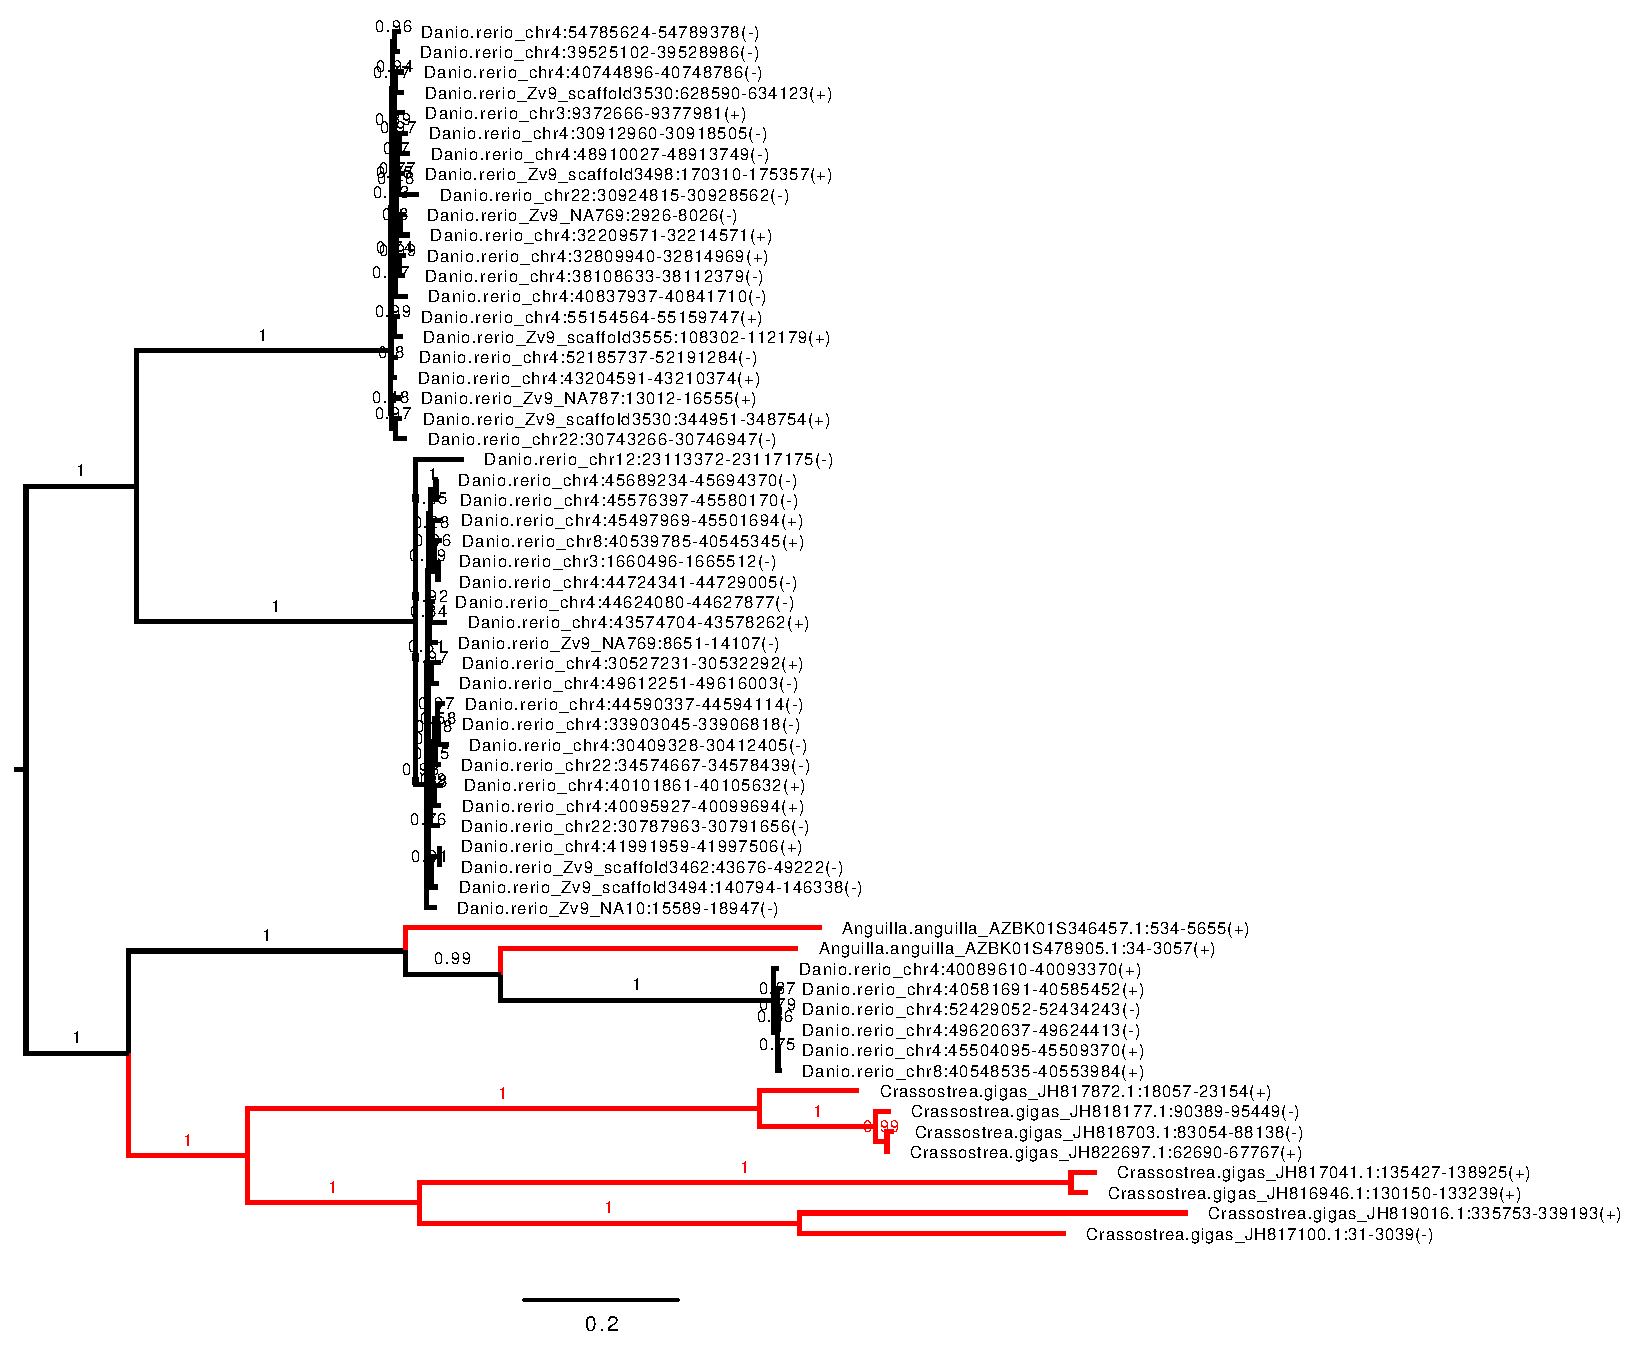
\includegraphics[scale=0.65]{suppFigures/clusters/c_25.pdf}
	\caption{\footnotesize \textbf{L1 cluster c\_25} \label{L1fam25}}
\end{figure}

\subsection*{L1 nucleotide ORFs}
%\addcontentsline{toc}{subsection}{L1 nucleotide ORFs}

\begin{figure}[H]
	\centering
	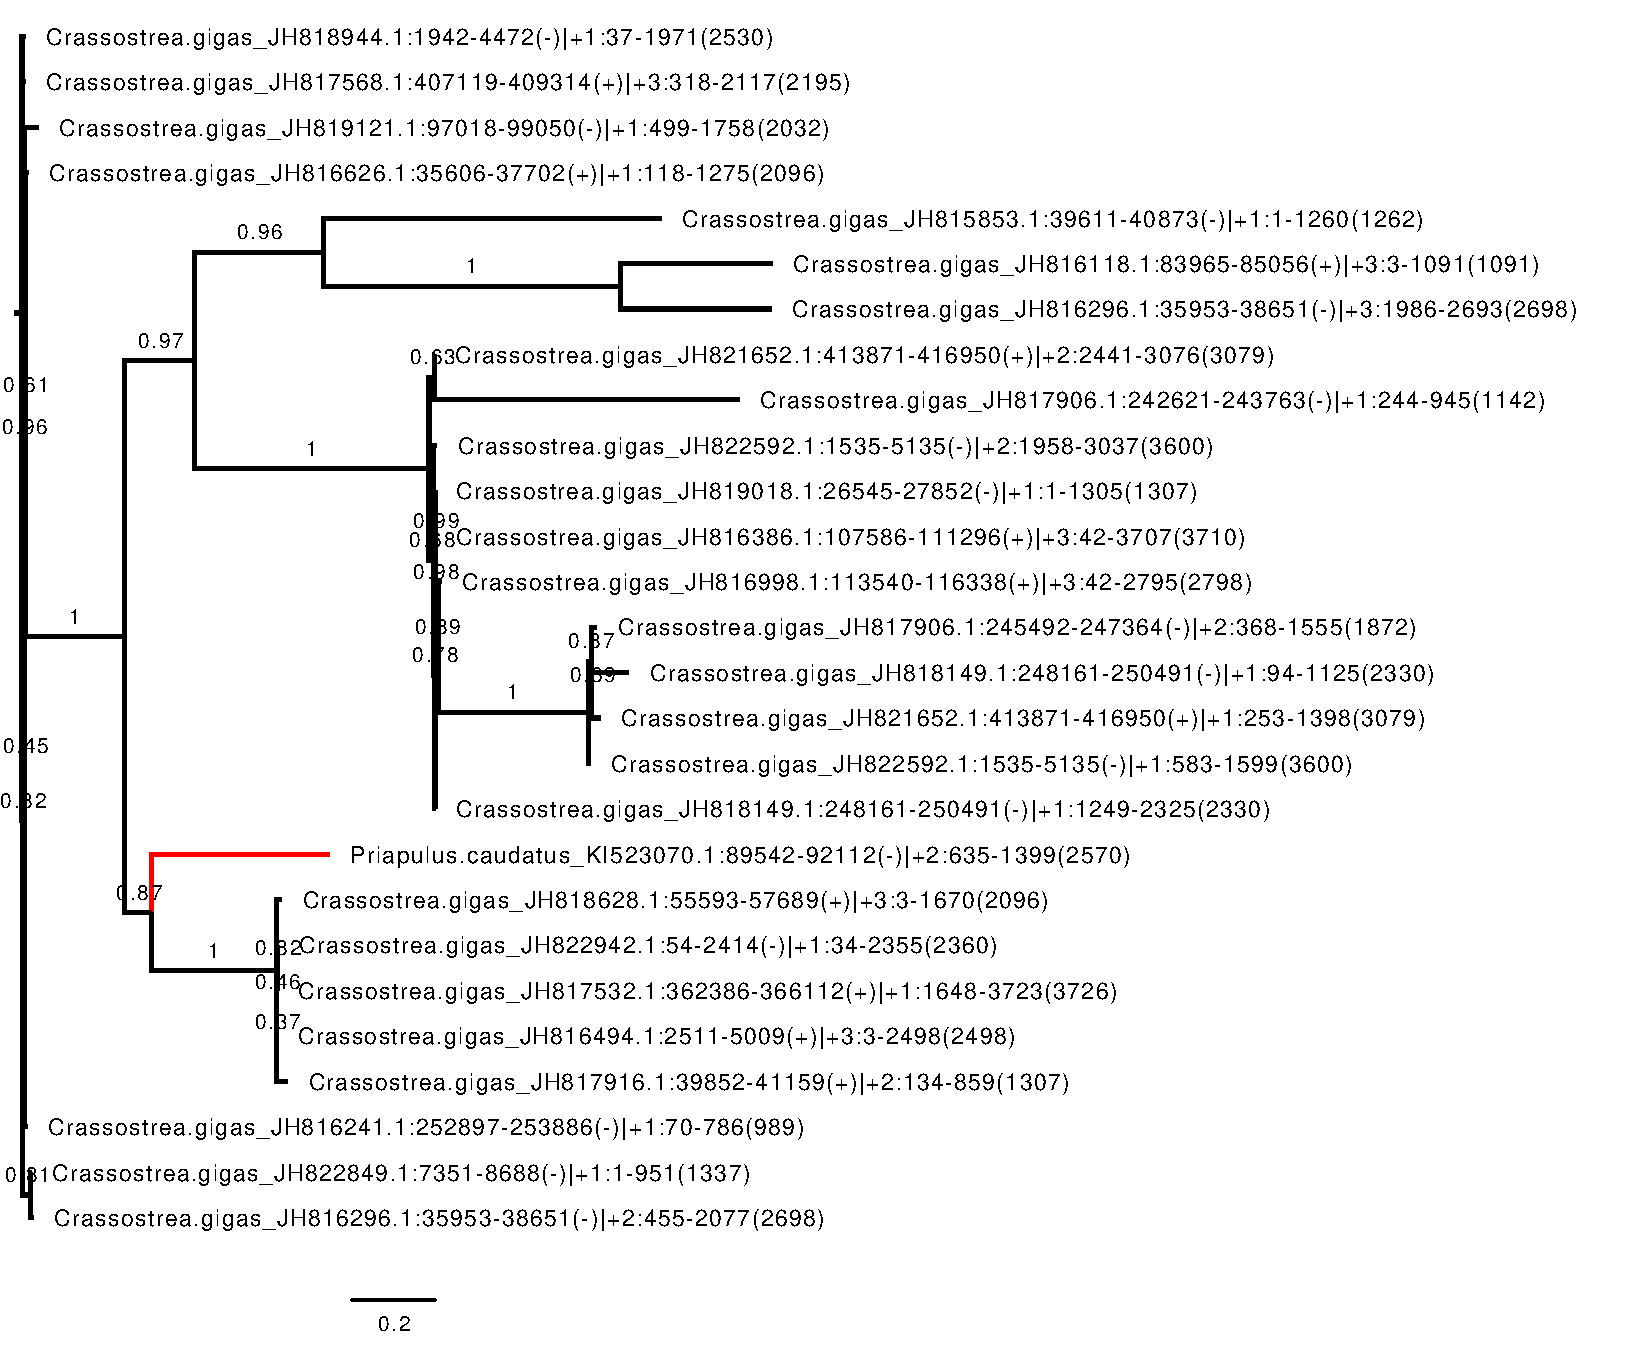
\includegraphics[scale=0.6]{suppFigures/clusters/c_666.pdf}
	\caption{\footnotesize \textbf{L1 cluster o\_666} \label{L1fam666}}
\end{figure}

\clearpage

\section*{Figures S3-54: Kimura divergence plots for BovB and L1}
\addcontentsline{toc}{section}{Figures S3-54: Kimura divergence plots for BovB and L1}
RepeatMasker divergence plots represent Kimura substitution levels of TEs against the RepBase super consensus library. 
For example, Figure 5b in the main text shows the RepeatMasker divergence plot for the cow (\textit{Bos taurus}), illustrating recent bursts of BovB and L1 activity in the genome with many copies sharing high identity to young, currently active elements.
\\ \\
The L1 superfamily includes both mammalian L1 elements (dark blue) and more diverse, frog-like Tx elements (light blue). 
Tx are typically found in fish, frogs and primitive eukaryotes (e.g. sea urchin \textit{Strongylocentrotus purpuratus}). 
BovB elements are coloured in orange.
\\ \\
Typically, species within a clade show consistent divergence patterns of both TEs (particularly if there has been little recent activity - see Chiroptera). 
Recently TE-active species, on the other hand, are likely to show bursts of seemingly random activity. Consider the plots for the two lizard species, \textit{Pogona vitticeps} and \textit{Anolis carolinensis}. \textit{Pogona} is implicated in many of the BovB HT events listed in Table S5, and this is supported by the huge burst of recent BovB activity shown in Figure~\ref{fig:Pogona_vitticeps}. This is also seen in all four snake species. In contrast, the \textit{Anolis} plot (Figure ~\ref{fig:Anolis_carolinensis}) indicates that L1s have become the dominant TE lineage in the genome. 
\\ \\
By estimating TE divergence from super consensus sequences, we can visualise the contrasting (and sometimes competing) dynamics of BovB and L1 elements over time. This is particularly important for species where BovB or L1 (or both) have taken off and accumulated quickly within the genome.

\subsection*{Marsupialia}
\addcontentsline{toc}{subsection}{Marsupialia}

\begin{figure}[H]
	\centering
	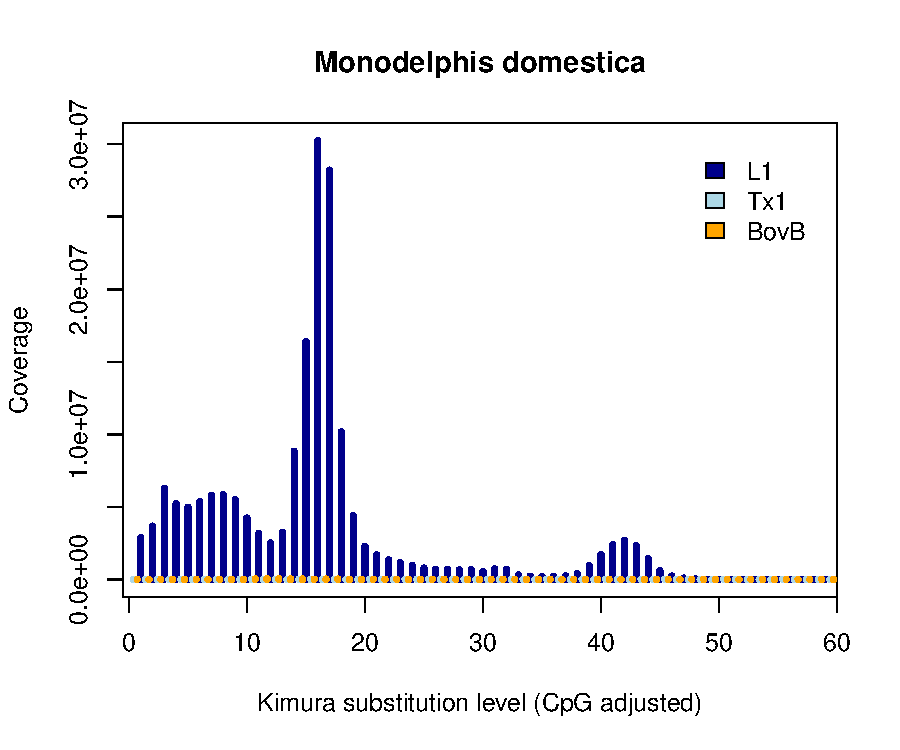
\includegraphics[scale=0.8]{suppFigures/divergencePlots/Monodelphis_domestica.pdf}
	\caption{\label{Monodelphis_domestica}}
\end{figure}

\begin{figure}[H]
	\centering
	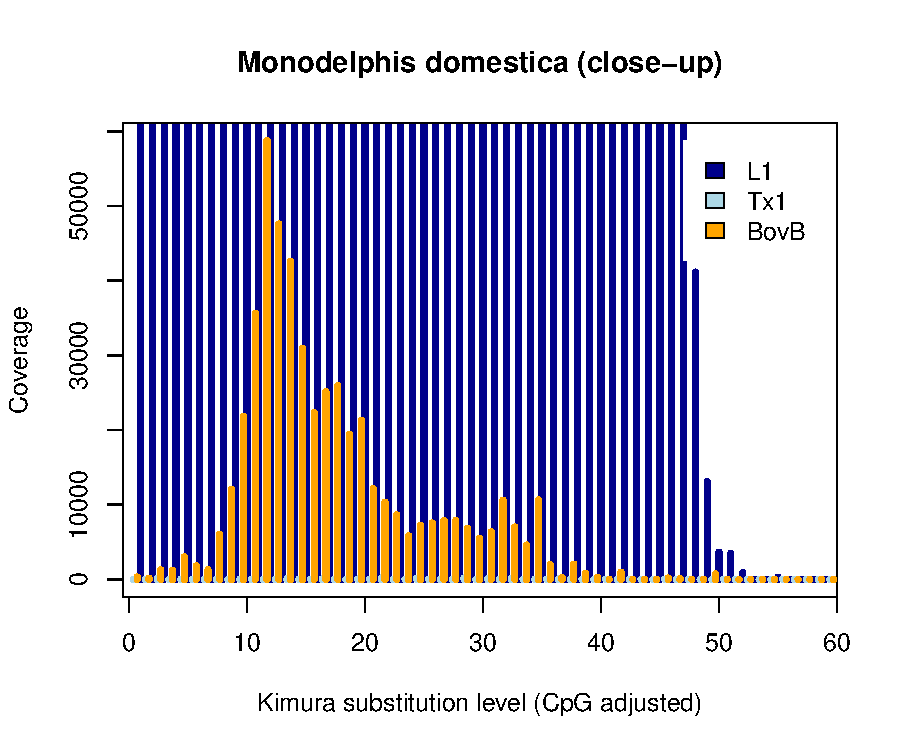
\includegraphics[scale=0.8]{suppFigures/divergencePlots/Monodelphis_domestica_closeup.pdf}
	\caption{\label{Monodelphis_domestica_closeup}}
\end{figure}

\begin{figure}[H]
	\centering
	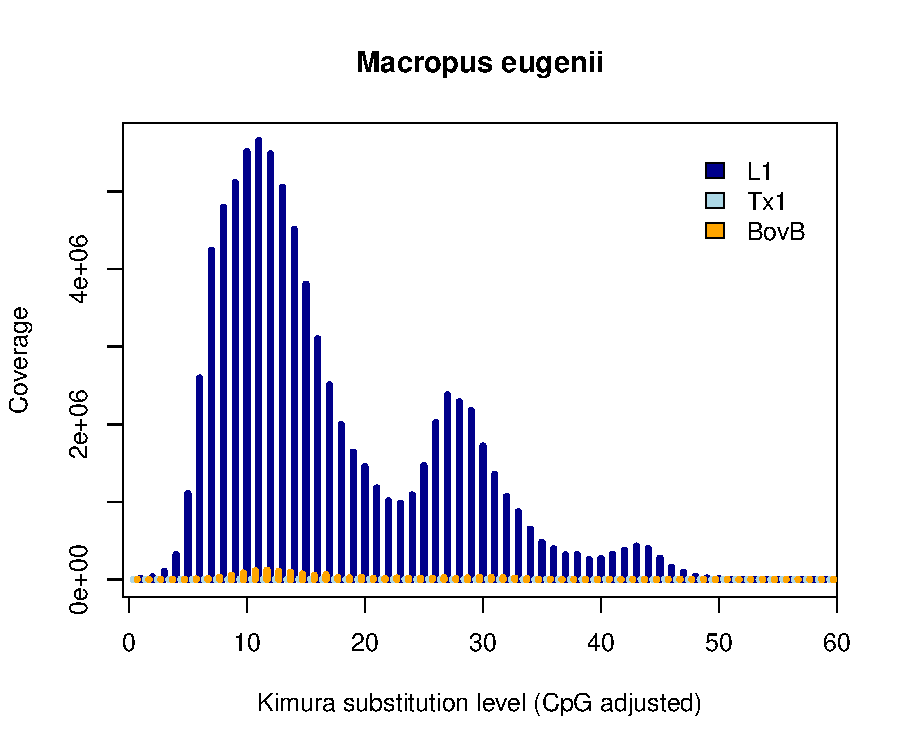
\includegraphics[scale=0.8]{suppFigures/divergencePlots/Macropus_eugenii.pdf}
	\caption{\label{Macropus_eugenii}}
\end{figure}

\begin{figure}[H]
	\centering
	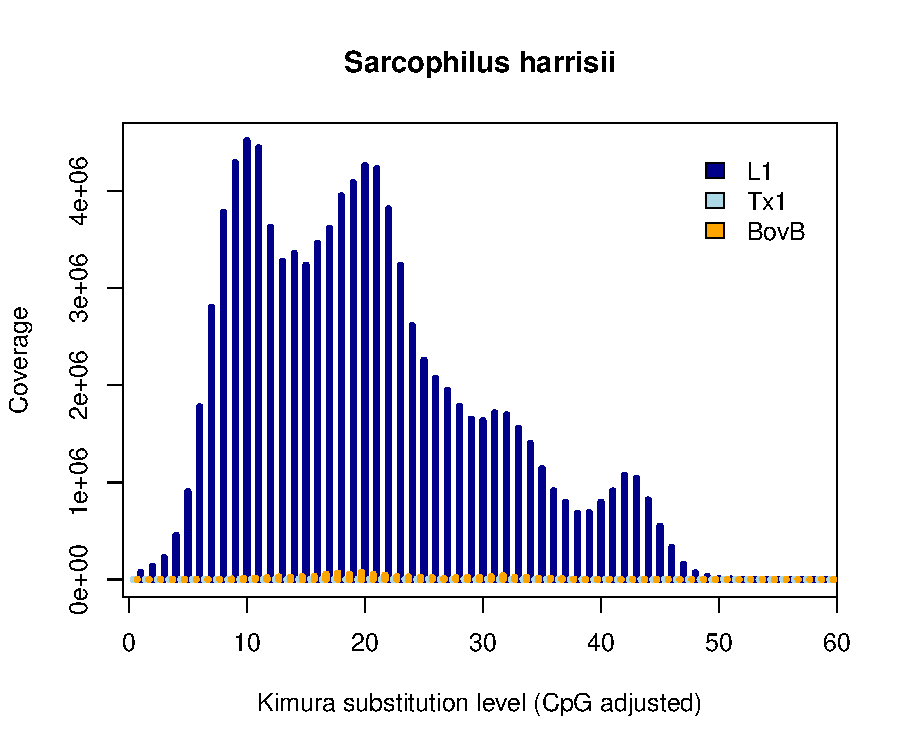
\includegraphics[scale=0.8]{suppFigures/divergencePlots/Sarcophilus_harrisii.pdf}
	\caption{\label{Sarcophilus_harrisii}}
\end{figure}

\subsection*{Afrotheria}
\addcontentsline{toc}{subsection}{Afrotheria}

\begin{figure}[H]
	\centering
	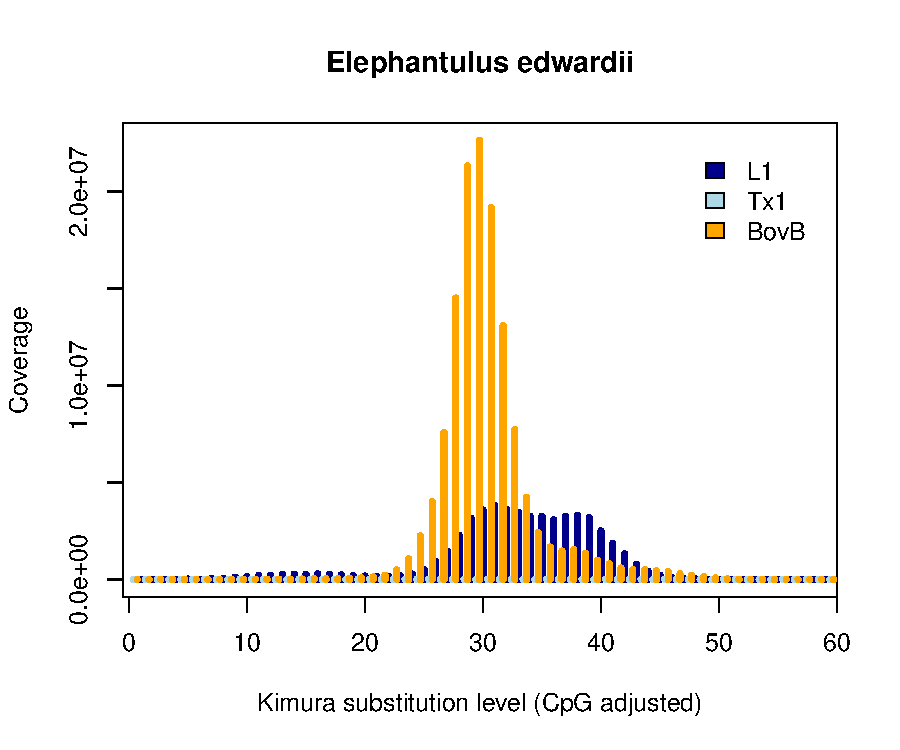
\includegraphics[scale=0.8]{suppFigures/divergencePlots/Elephantulus_edwardii.pdf}
	\caption{\label{Elephantulus_edwardii}}
\end{figure}

\begin{figure}[H]
	\centering
	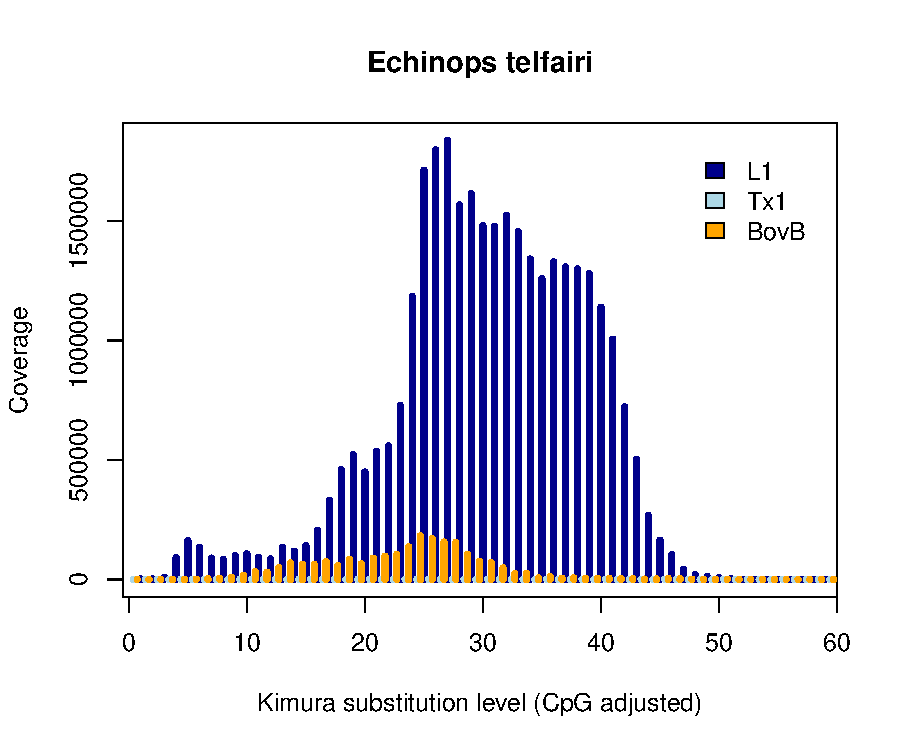
\includegraphics[scale=0.8]{suppFigures/divergencePlots/Echinops_telfairi.pdf}
	\caption{\label{Echinops_telfairi}}
\end{figure}

\begin{figure}[H]
	\centering
	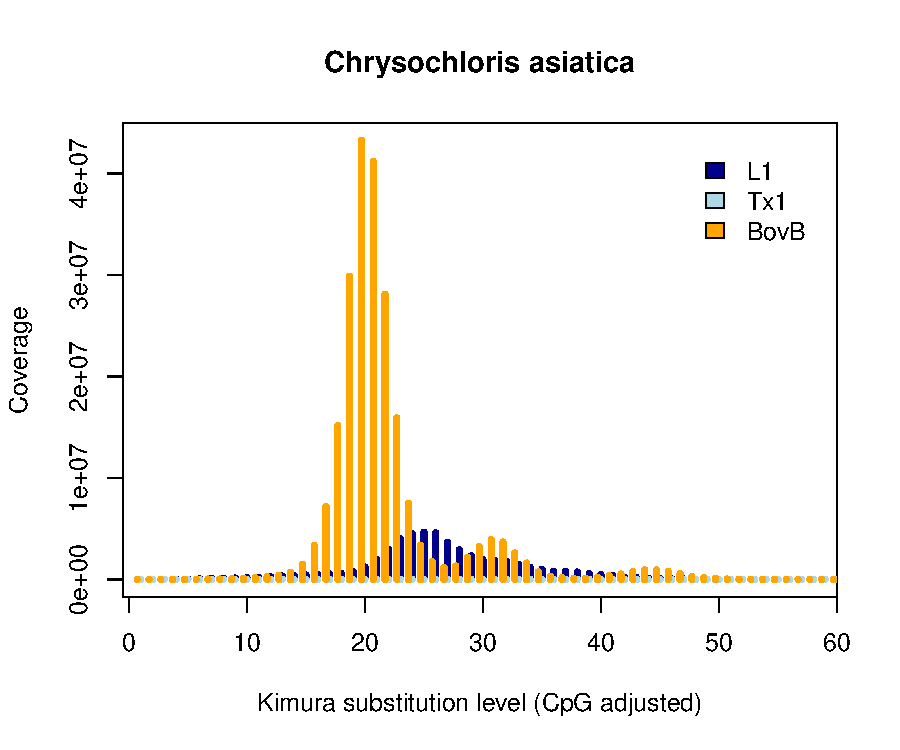
\includegraphics[scale=0.8]{suppFigures/divergencePlots/Chrysochloris_asiatica.pdf}
	\caption{\label{Chrysochloris}}
\end{figure}

\begin{figure}[H]
	\centering
	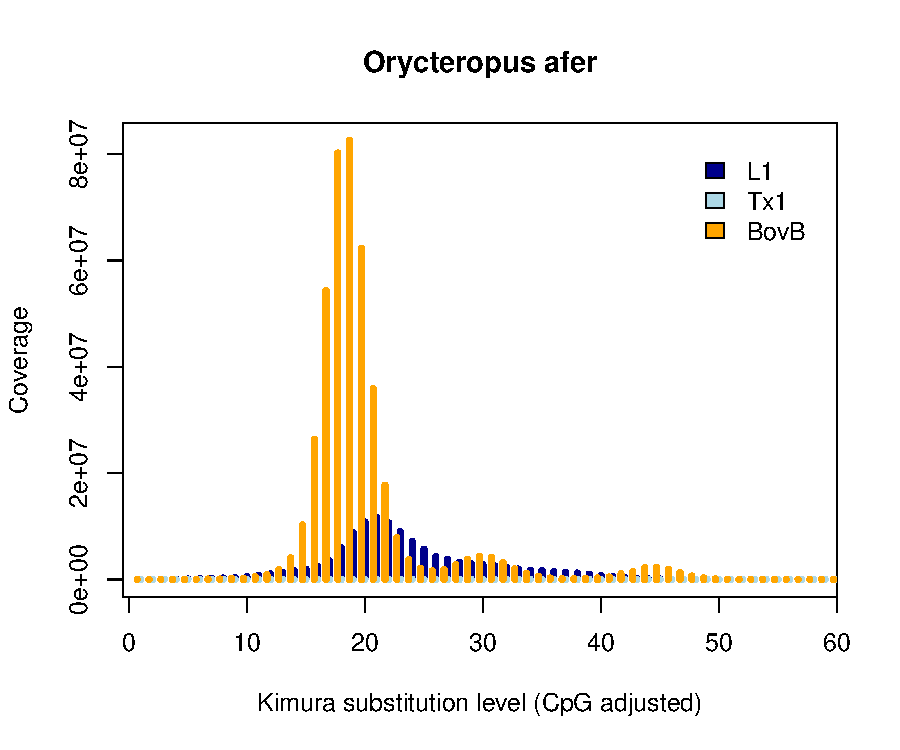
\includegraphics[scale=0.8]{suppFigures/divergencePlots/Orycteropus_afer.pdf}
	\caption{\label{Orycteropus}}
\end{figure}

\begin{figure}[H]
	\centering
	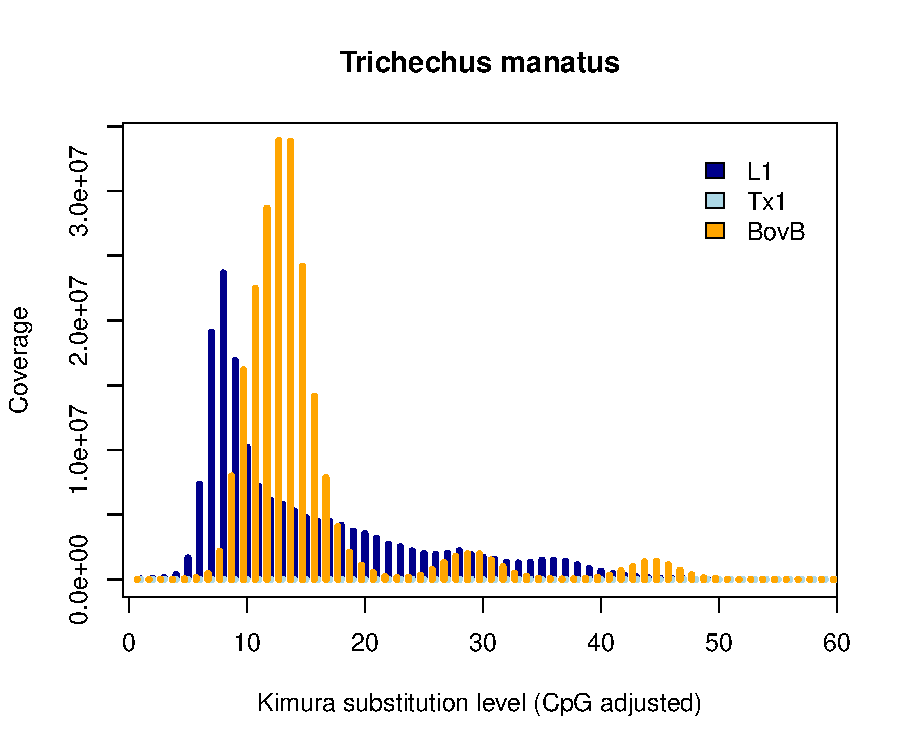
\includegraphics[scale=0.8]{suppFigures/divergencePlots/Trichechus_manatus.pdf}
	\caption{\label{Trichchus}}
\end{figure}

\begin{figure}[H]
	\centering
	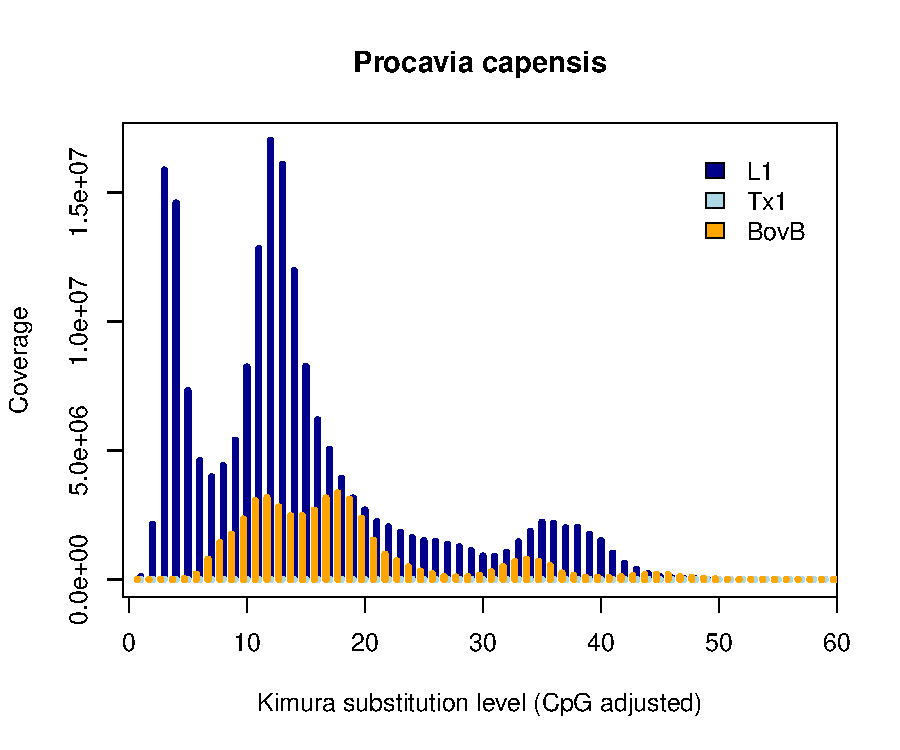
\includegraphics[scale=0.8]{suppFigures/divergencePlots/Procavia_capensis.pdf}
	\caption{\label{Procavia}}
\end{figure}

\begin{figure}[H]
	\centering
	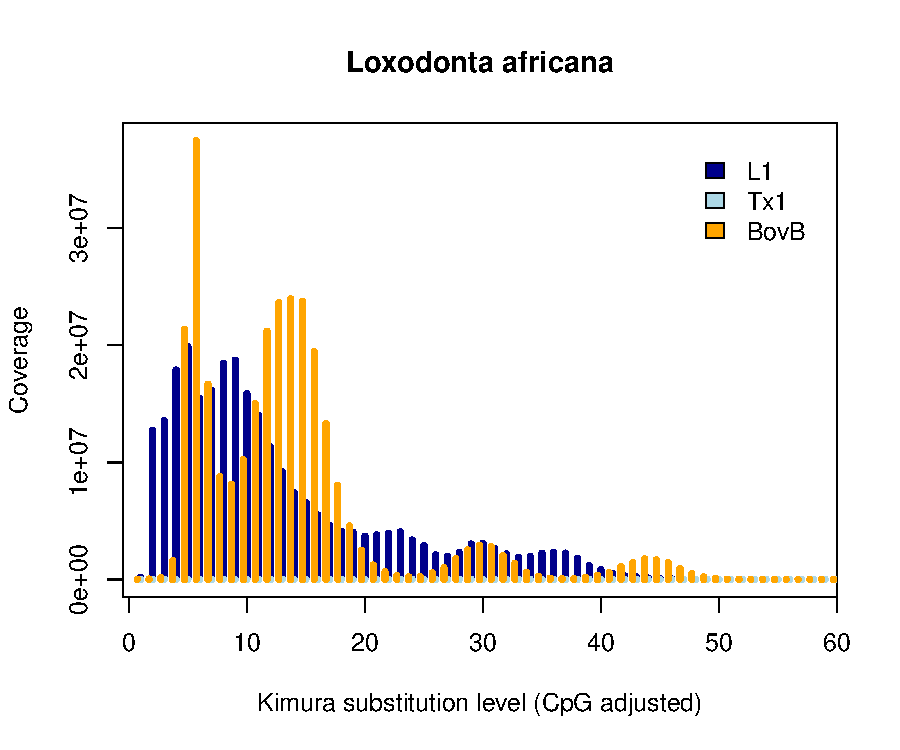
\includegraphics[scale=0.8]{suppFigures/divergencePlots/Loxodonta_africana.pdf}
	\caption{\label{Loxodonta}}
\end{figure}

\subsection*{Chiroptera}
\addcontentsline{toc}{subsection}{Chiroptera}

\begin{figure}[H]
	\centering
	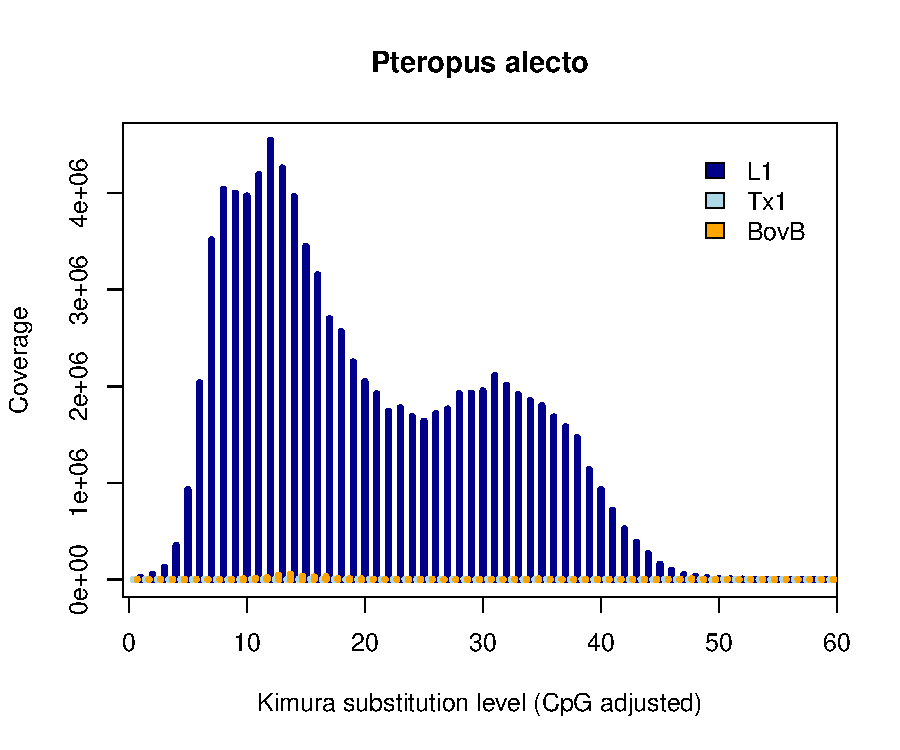
\includegraphics[scale=0.8]{suppFigures/divergencePlots/Pteropus_alecto.pdf}
	\caption{\label{Pteropus_alecto}}
\end{figure}

\begin{figure}[H]
	\centering
	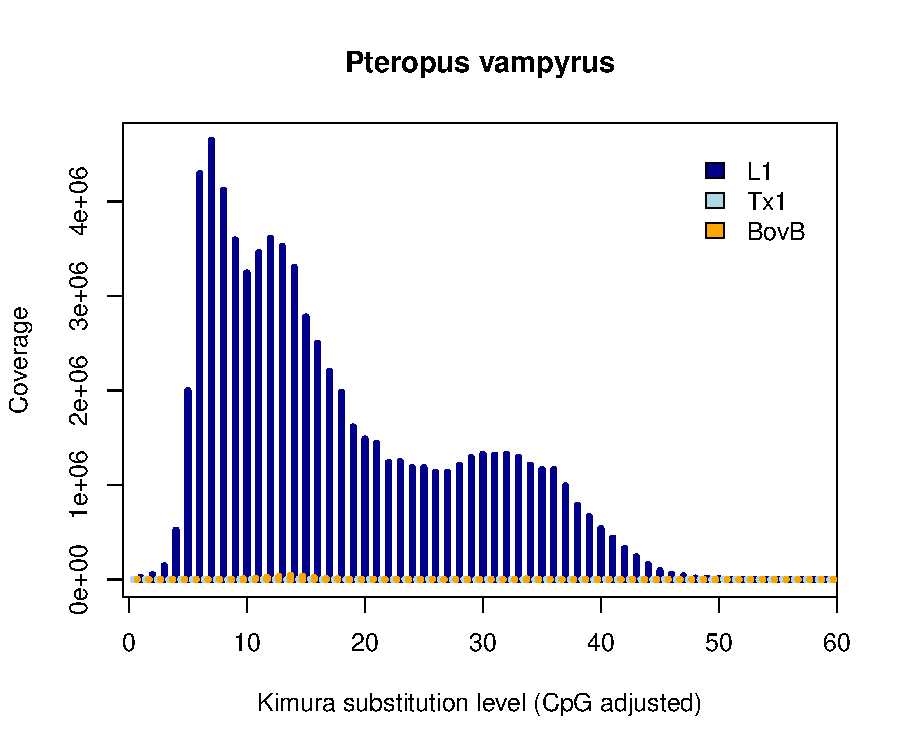
\includegraphics[scale=0.8]{suppFigures/divergencePlots/Pteropus_vampyrus.pdf}
	\caption{\label{Pteropus_vampyrus}}
\end{figure}

\begin{figure}[H]
	\centering
	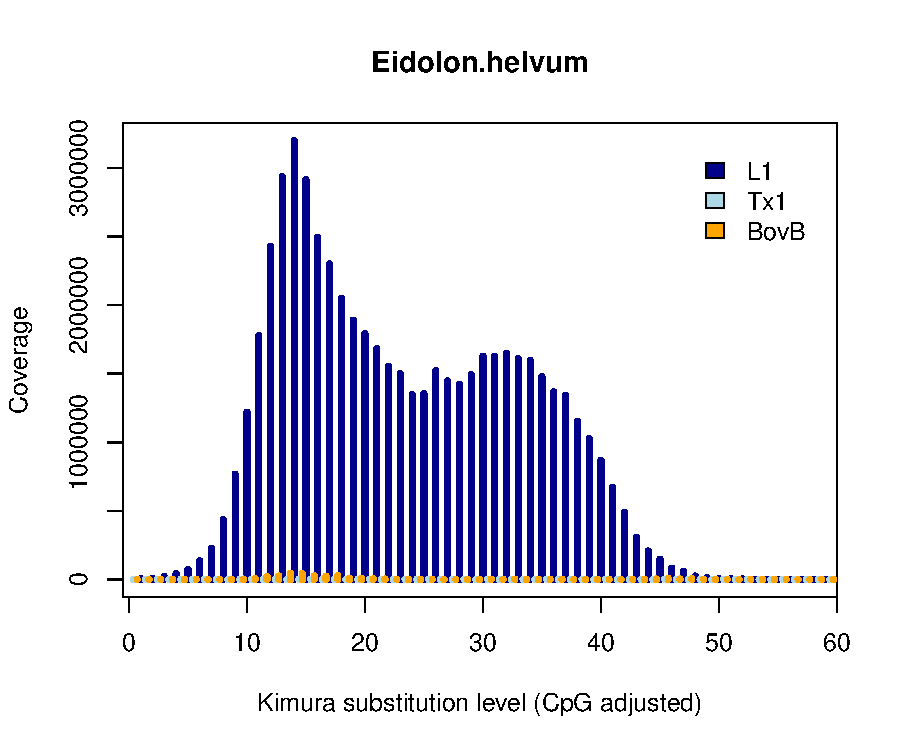
\includegraphics[scale=0.8]{suppFigures/divergencePlots/Eidolon_helvum.pdf}
	\caption{\label{Eidolon_helvum}}
\end{figure}

\begin{figure}[H]
	\centering
	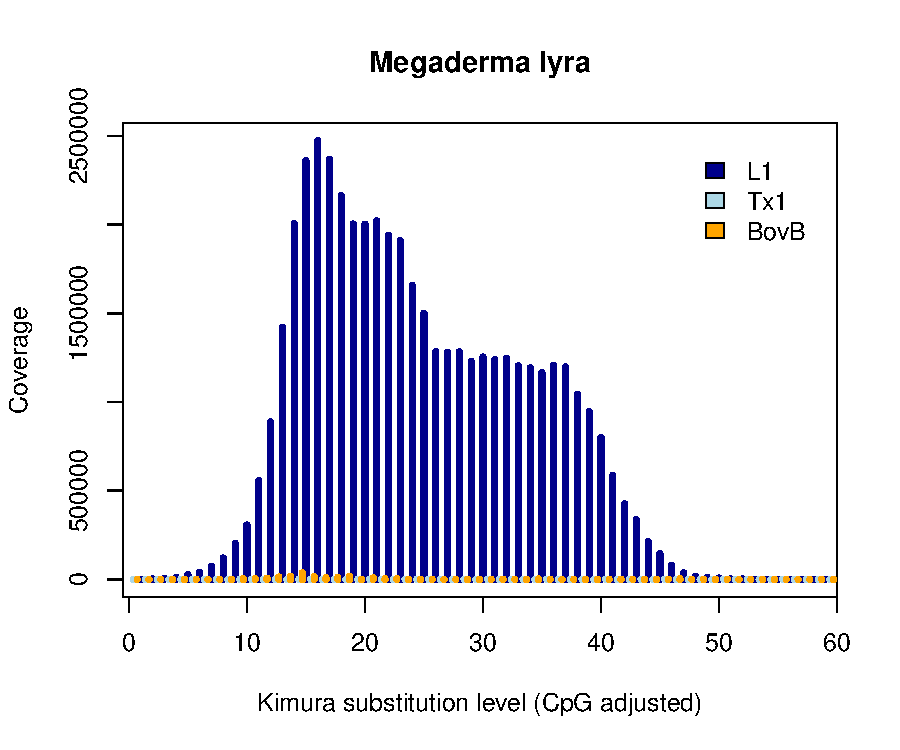
\includegraphics[scale=0.8]{suppFigures/divergencePlots/Megaderma_lyra.pdf}
	\caption{\label{Megaderma_lyra}}
\end{figure}

\begin{figure}[H]
	\centering
	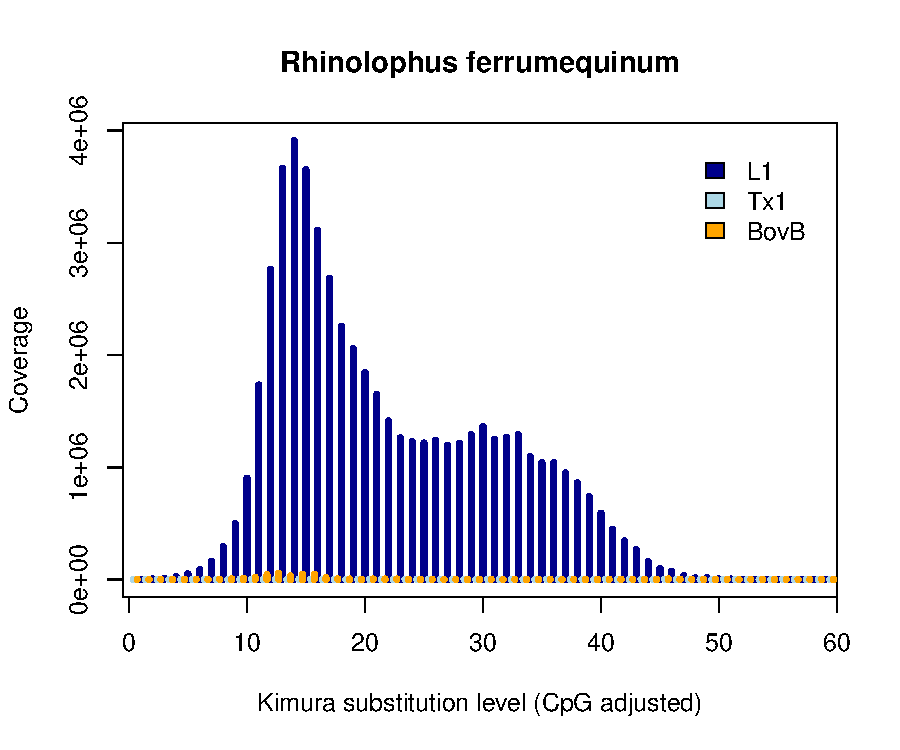
\includegraphics[scale=0.8]{suppFigures/divergencePlots/Rhinolophus_ferrumequinum.pdf}
	\caption{\label{Rhinolophus_ferrumequinum}}
\end{figure}

\begin{figure}[H]
	\centering
	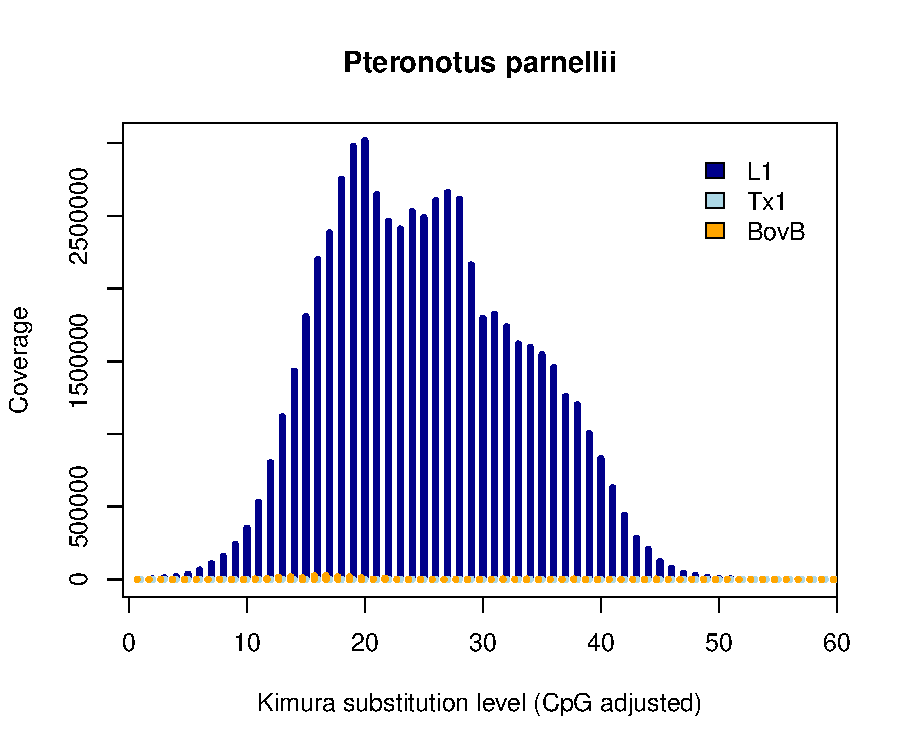
\includegraphics[scale=0.8]{suppFigures/divergencePlots/Pteronotus_parnellii.pdf}
	\caption{\label{Pteronotus_parnellii}}
\end{figure}

\begin{figure}[H]
	\centering
	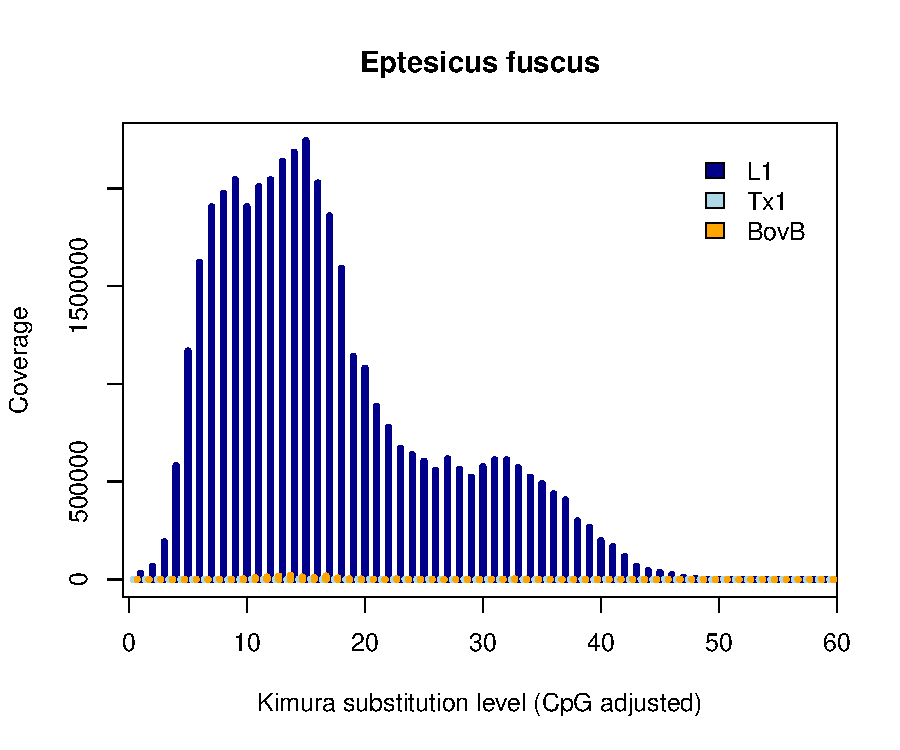
\includegraphics[scale=0.8]{suppFigures/divergencePlots/Eptesicus_fuscus.pdf}
	\caption{\label{Eptesicus_fuscus}}
\end{figure}

\begin{figure}[H]
	\centering
	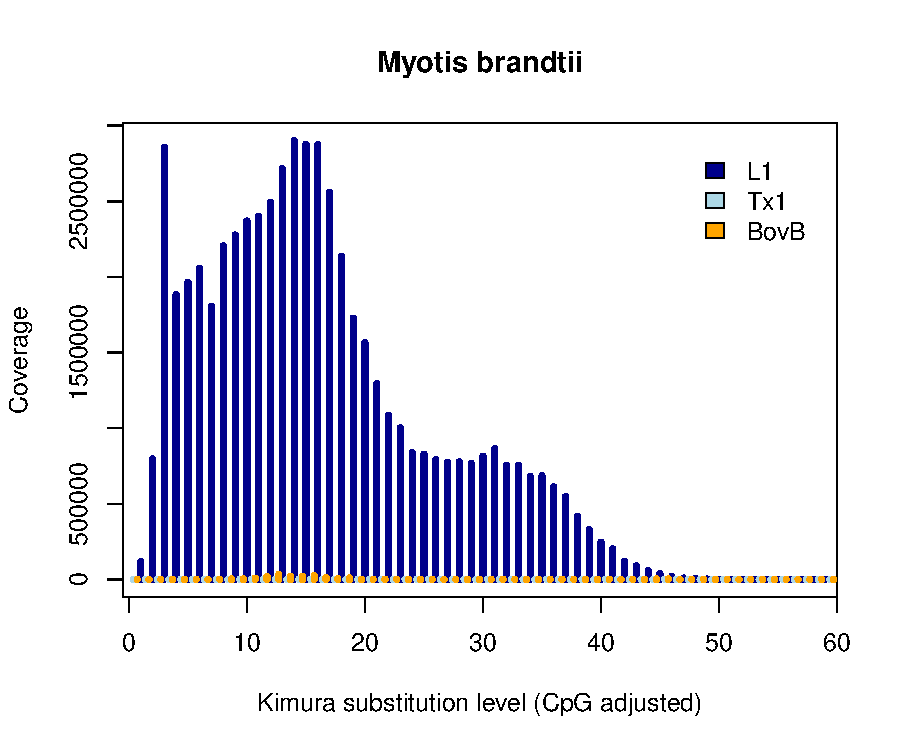
\includegraphics[scale=0.8]{suppFigures/divergencePlots/Myotis_brandtii.pdf}
	\caption{\label{Myotis_brandtii}}
\end{figure}

\begin{figure}[H]
	\centering
	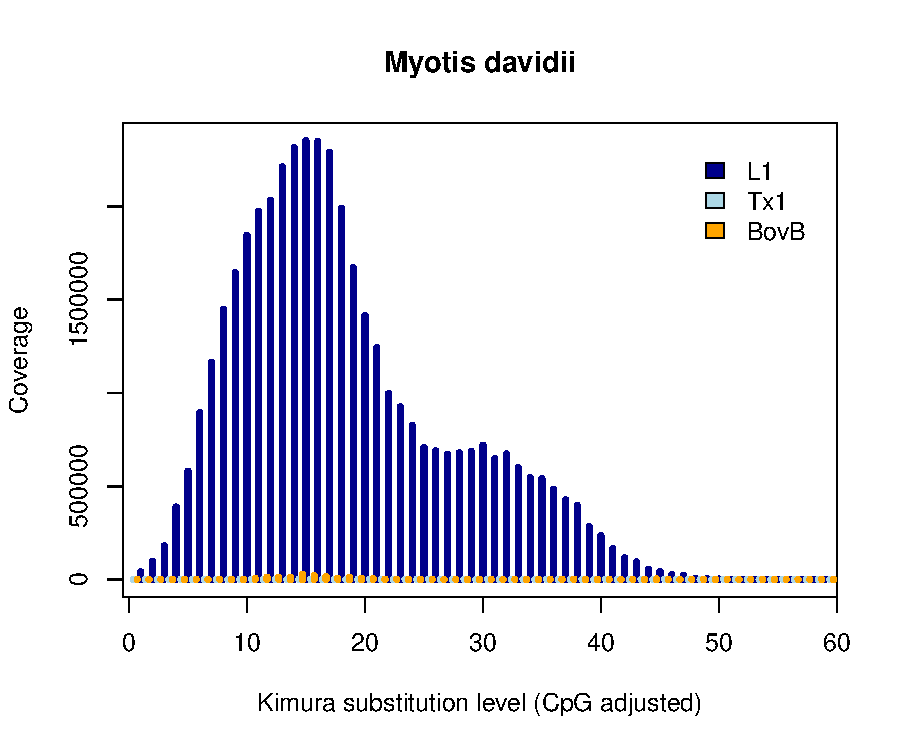
\includegraphics[scale=0.8]{suppFigures/divergencePlots/Myotis_davidii.pdf}
	\caption{\label{Myotis_davidii}}
\end{figure}

\begin{figure}[H]
	\centering
	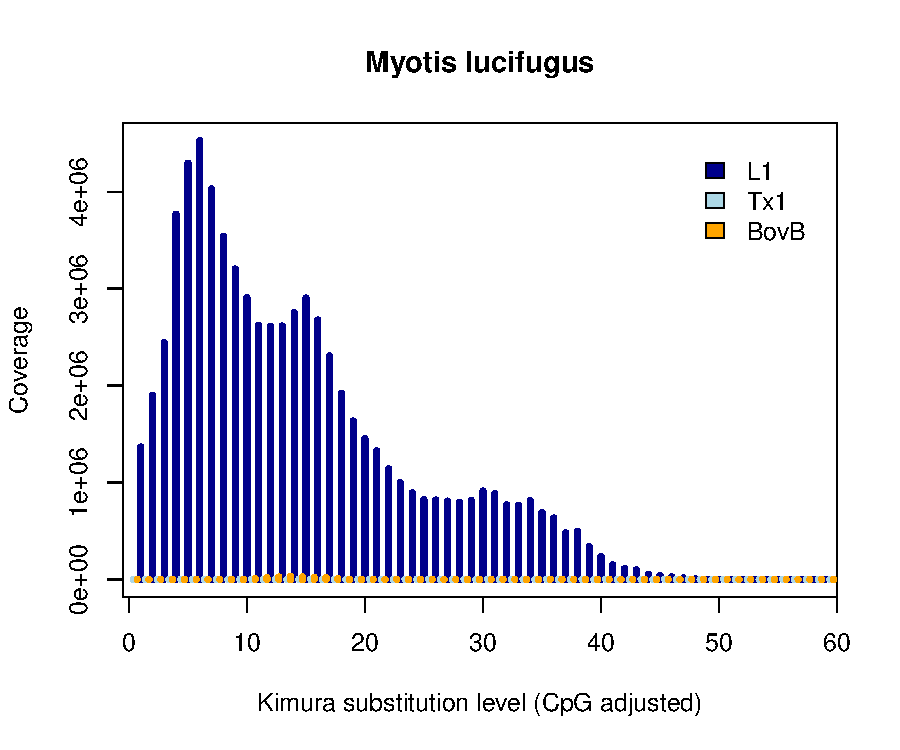
\includegraphics[scale=0.8]{suppFigures/divergencePlots/Myotis_lucifugus.pdf}
	\caption{\label{Myotis_lucifugus}}
\end{figure}

\begin{figure}[H]
	\centering
	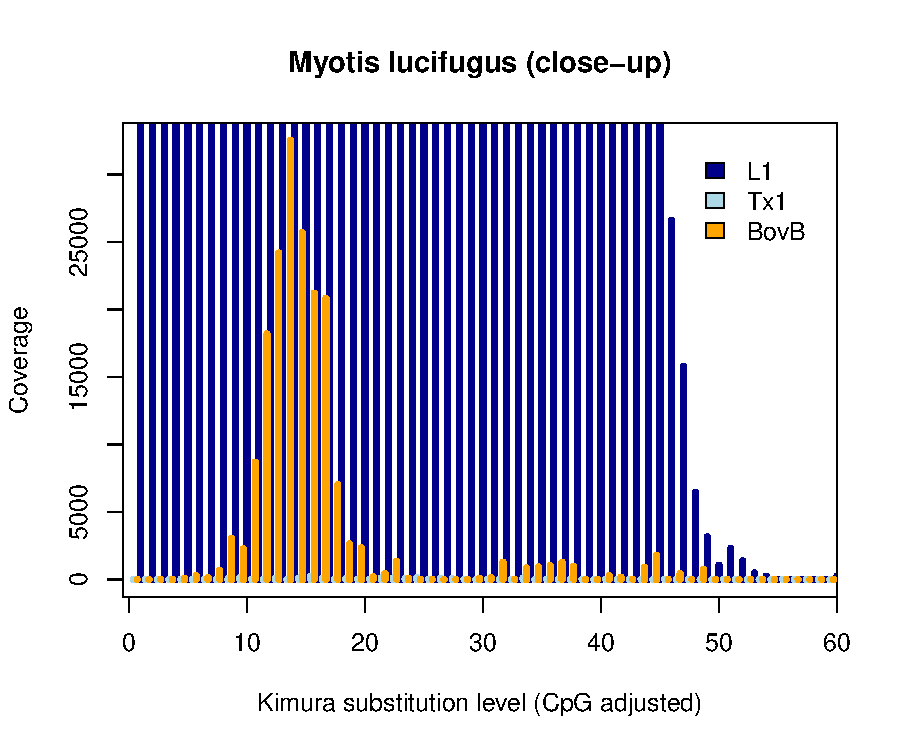
\includegraphics[scale=0.8]{suppFigures/divergencePlots/Myotis_lucifugus_closeup.pdf}
	\caption{\label{Myotis_lucifugus_closeup}}
\end{figure}

\subsection*{Perissodactyla}
\addcontentsline{toc}{subsection}{Perissodactyla}

\begin{figure}[H]
	\centering
	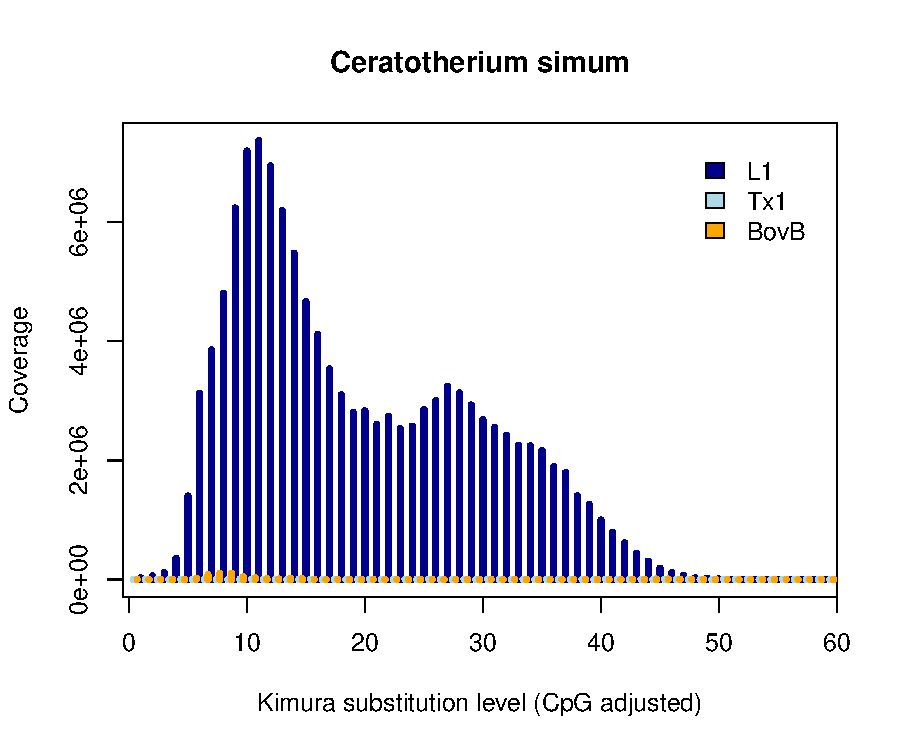
\includegraphics[scale=0.8]{suppFigures/divergencePlots/Ceratotherium_simum.pdf}
	\caption{\label{Ceratotherium_simum}}
\end{figure}

\begin{figure}[H]
	\centering
	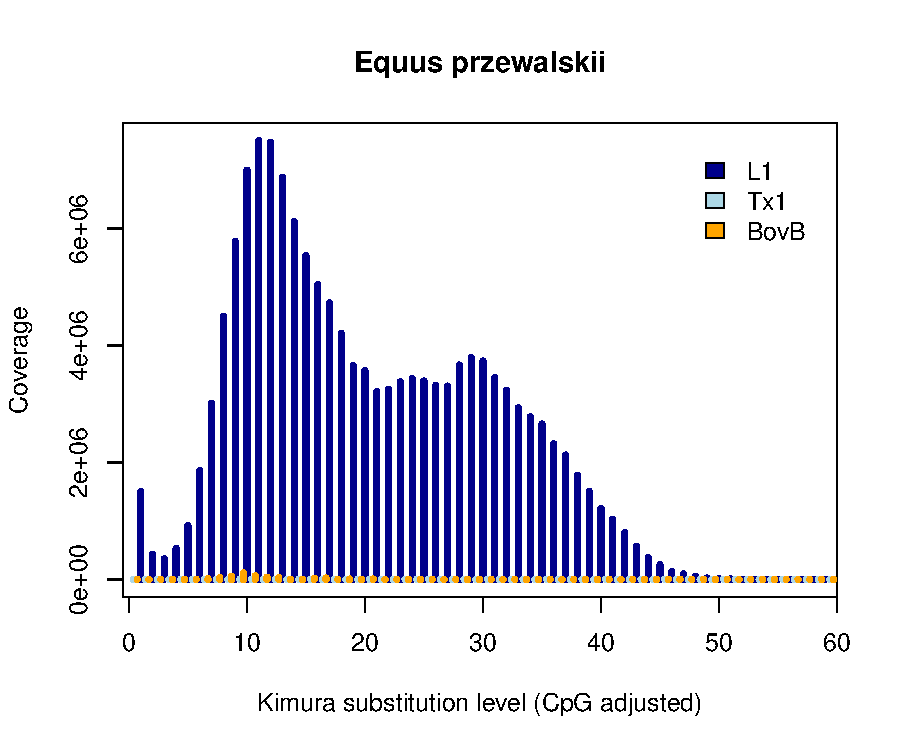
\includegraphics[scale=0.8]{suppFigures/divergencePlots/Equus_przewalskii.pdf}
	\caption{\label{Equus_przewalskii}}
\end{figure}

\begin{figure}[H]
	\centering
	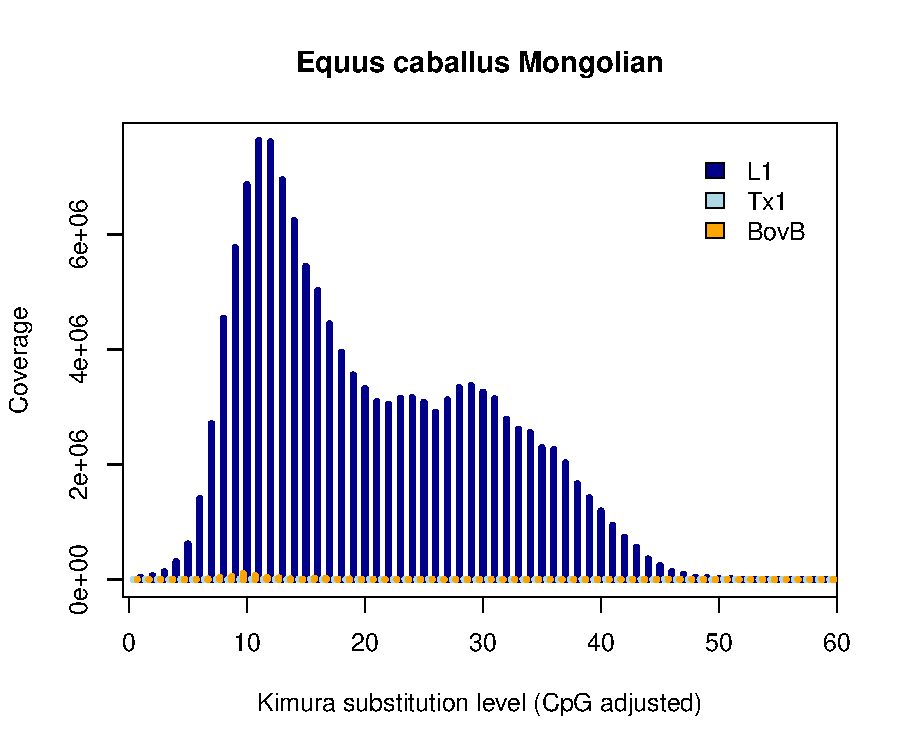
\includegraphics[scale=0.8]{suppFigures/divergencePlots/Equus_caballus_Mongolian.pdf}
	\caption{\label{Equus_caballus_Mongolian}}
\end{figure}

\begin{figure}[H]
	\centering
	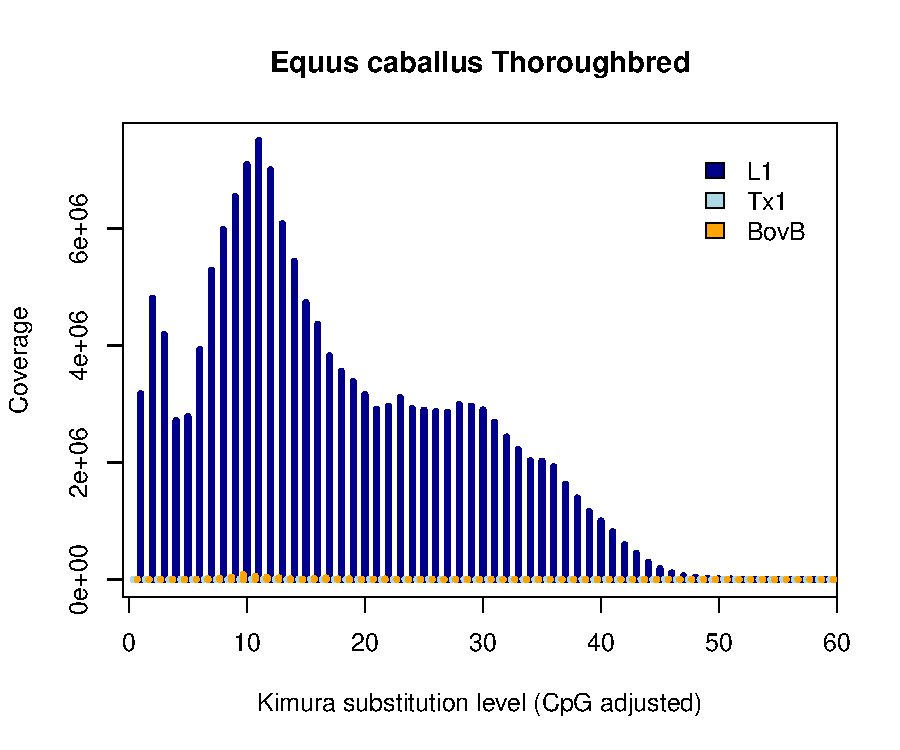
\includegraphics[scale=0.8]{suppFigures/divergencePlots/Equus_caballus_Thoroughbred.pdf}
	\caption{\label{Equus_caballus_Thoroughbred}}
\end{figure}

\begin{figure}[H]
	\centering
	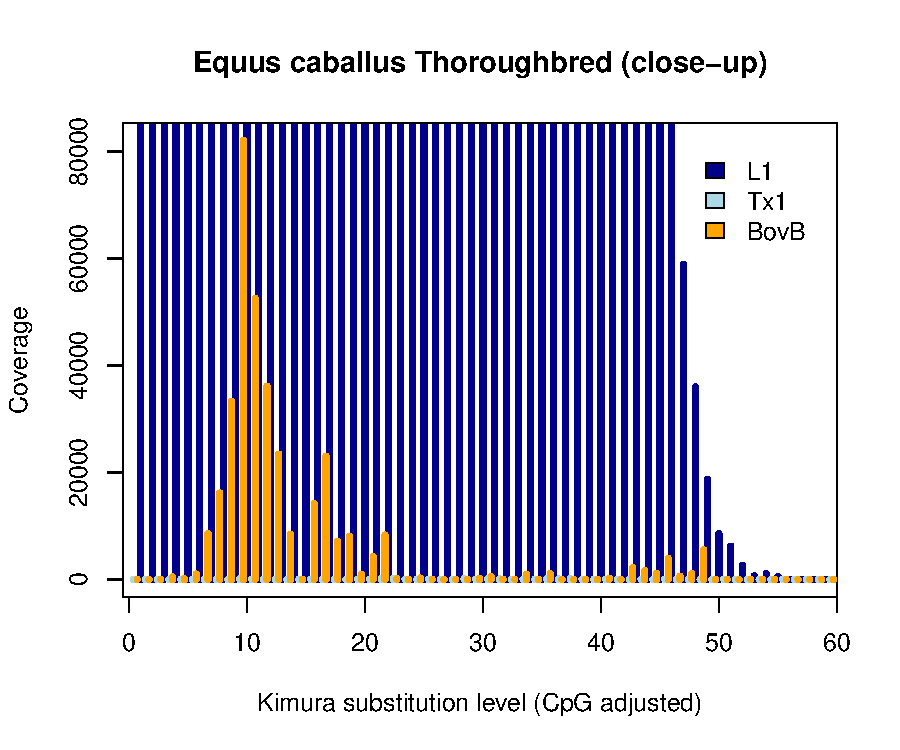
\includegraphics[scale=0.8]{suppFigures/divergencePlots/Equus_caballus_Thoroughbred_closeup.pdf}
	\caption{\label{Equus_caballus_Thoroughbred_closeup}}
\end{figure}

\subsection*{Bovidae}
\addcontentsline{toc}{subsection}{Bovidae}

\begin{figure}[H]
	\centering
	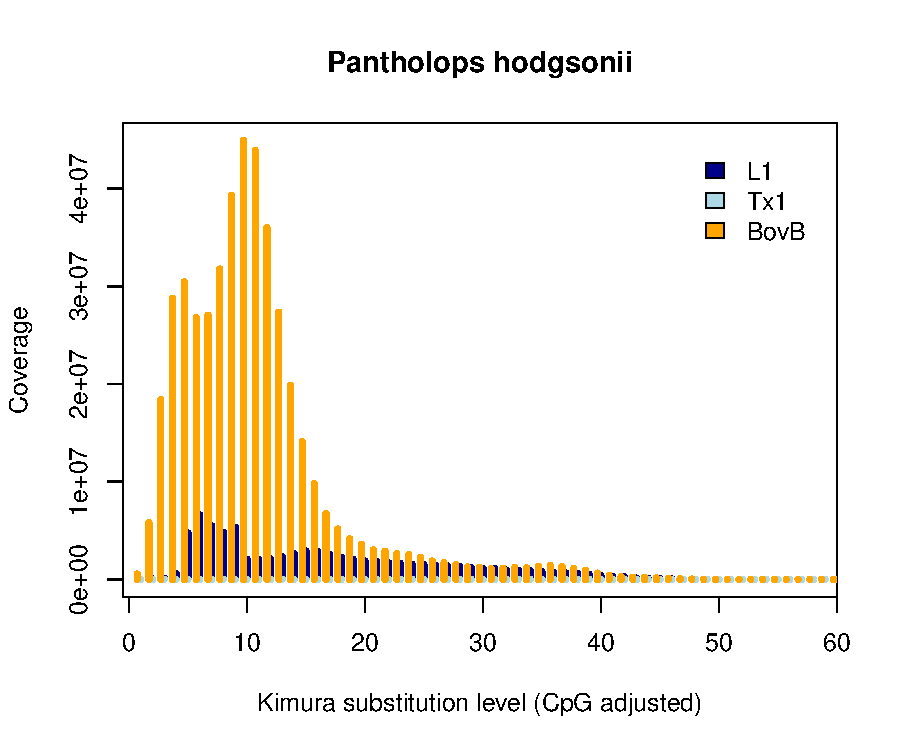
\includegraphics[scale=0.8]{suppFigures/divergencePlots/Pantholops_hodgsonii.pdf}
	\caption{\label{Pantholops}}
\end{figure}

\begin{figure}[H]
	\centering
	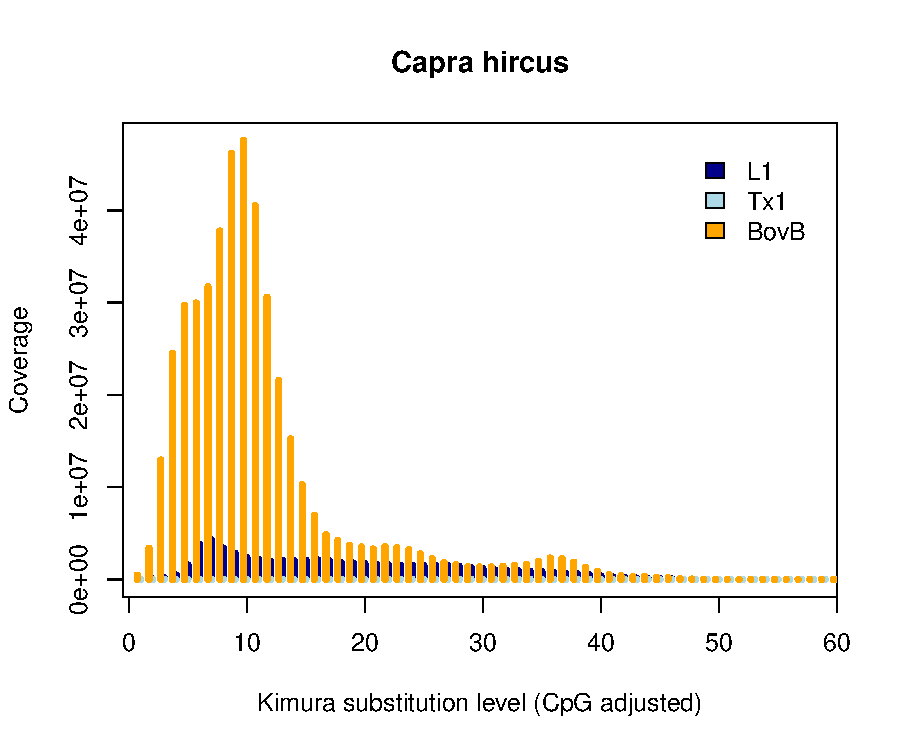
\includegraphics[scale=0.8]{suppFigures/divergencePlots/Capra_hircus.pdf}
	\caption{\label{Capra}}
\end{figure}

\begin{figure}[H]
	\centering
	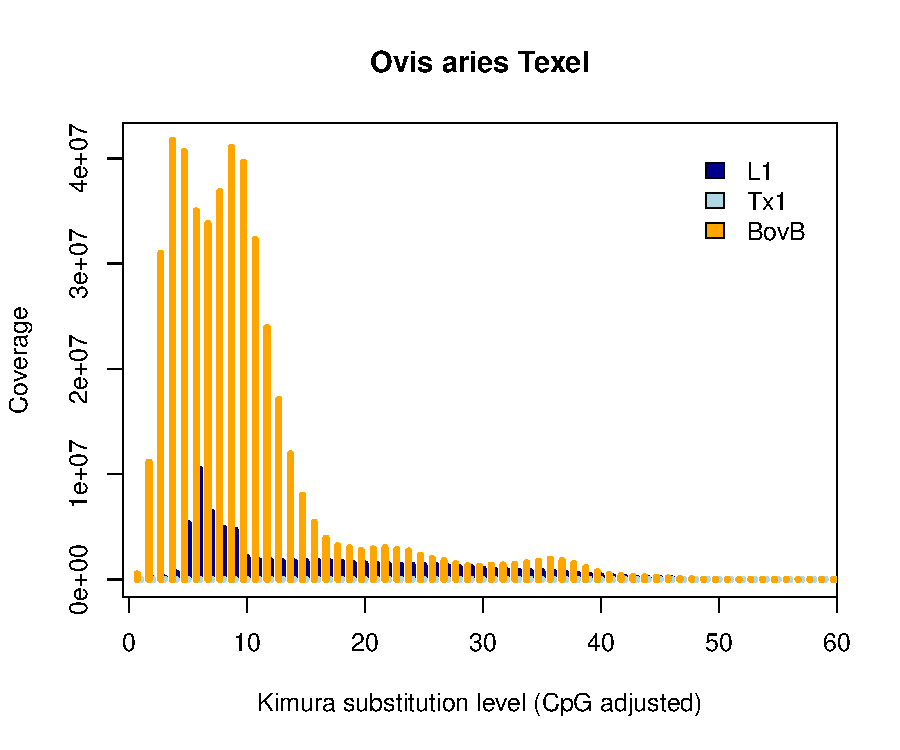
\includegraphics[scale=0.8]{suppFigures/divergencePlots/Ovis_aries_Texel.pdf}
	\caption{\label{OvisT}}
\end{figure}

\begin{figure}[H]
	\centering
	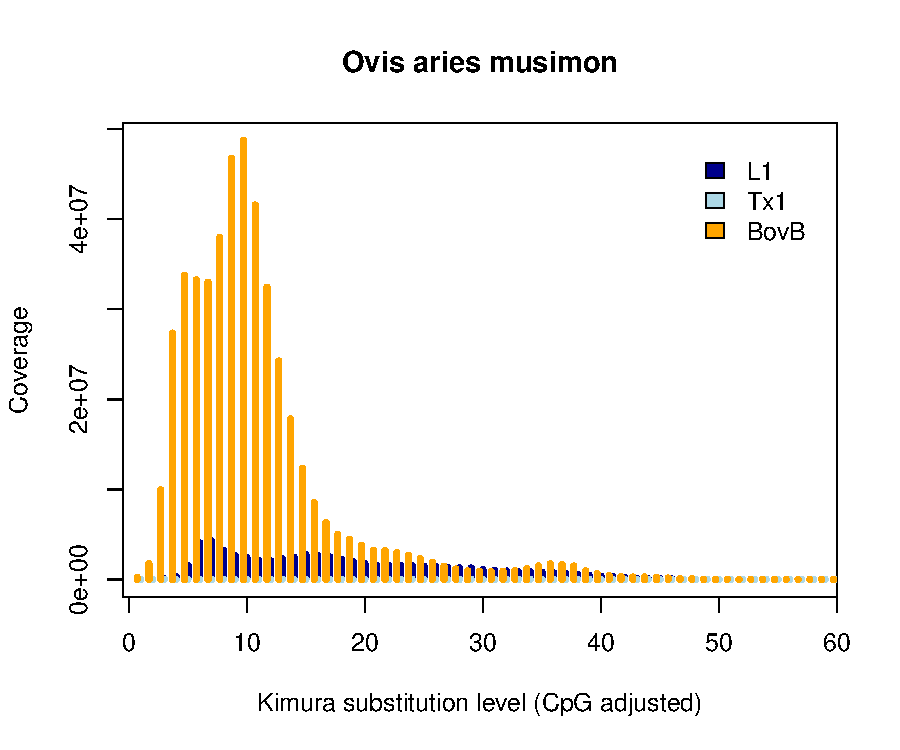
\includegraphics[scale=0.8]{suppFigures/divergencePlots/Ovis_aries_musimon.pdf}
	\caption{\label{OvisM}}
\end{figure}

\begin{figure}[H]
	\centering
	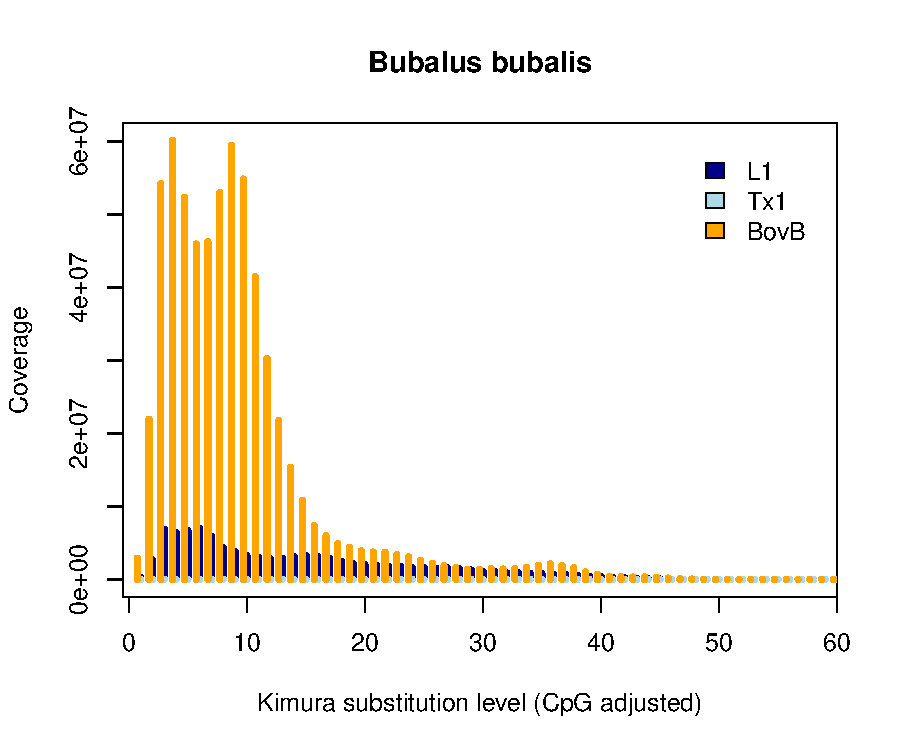
\includegraphics[scale=0.8]{suppFigures/divergencePlots/Bubalus_bubalis.pdf}
	\caption{\label{Bubulus}}
\end{figure}

\begin{figure}[H]
	\centering
	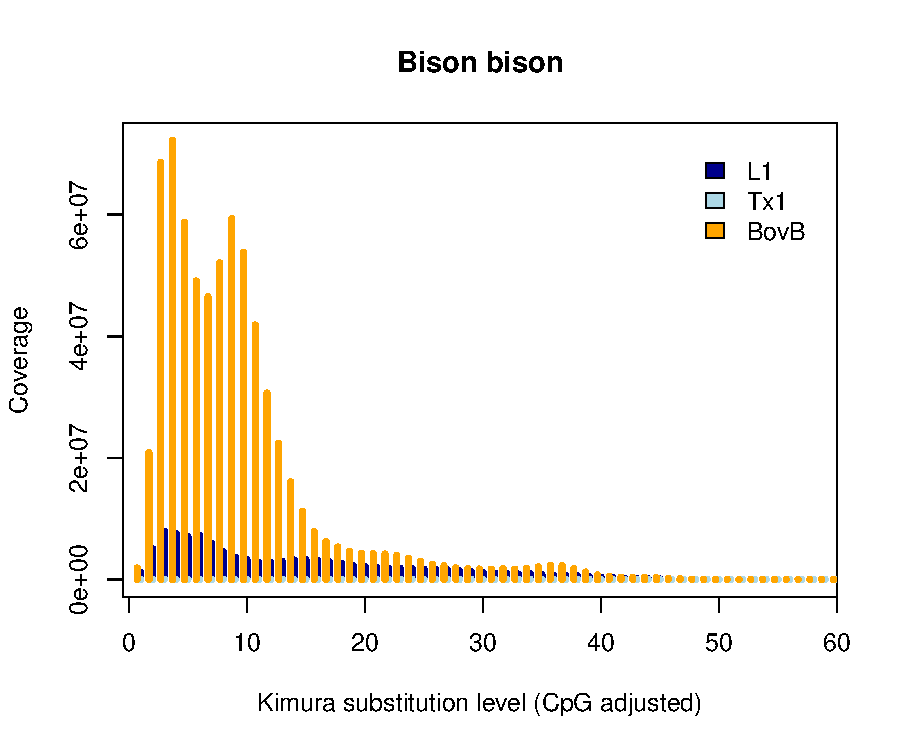
\includegraphics[scale=0.8]{suppFigures/divergencePlots/Bison_bison.pdf}
	\caption{\label{Bison}}
\end{figure}

\begin{figure}[H]
	\centering
	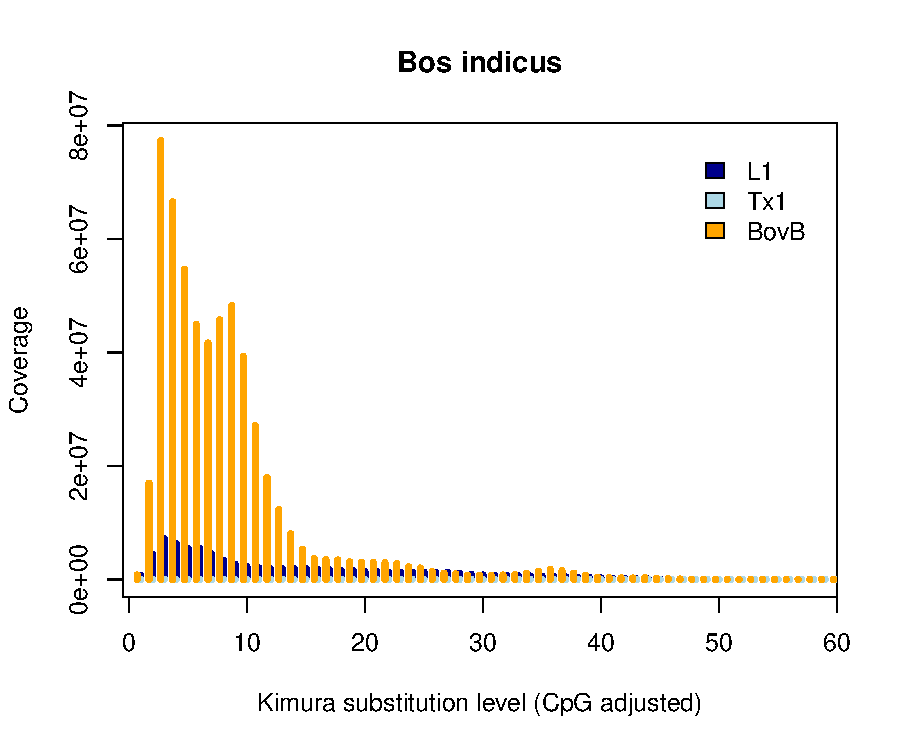
\includegraphics[scale=0.8]{suppFigures/divergencePlots/Bos_indicus.pdf}
	\caption{\label{BosI}}
\end{figure}

\begin{figure}[H]
	\centering
	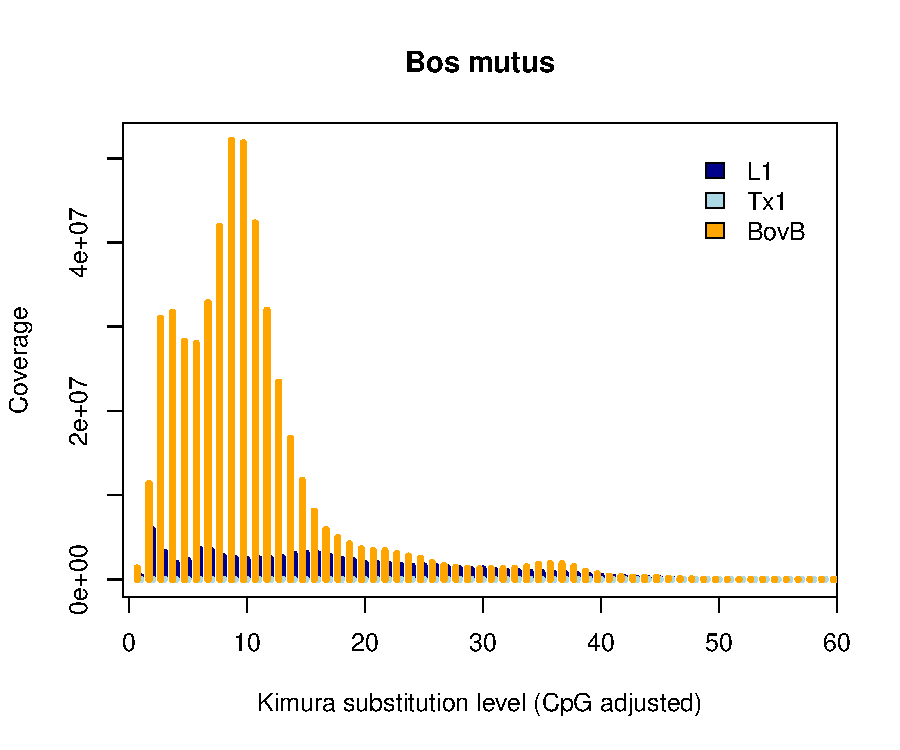
\includegraphics[scale=0.8]{suppFigures/divergencePlots/Bos_mutus.pdf}
	\caption{\label{BosM}}
\end{figure}

\subsection*{Squamata}
\addcontentsline{toc}{subsection}{Squamata}

\begin{figure}[H]
	\centering
	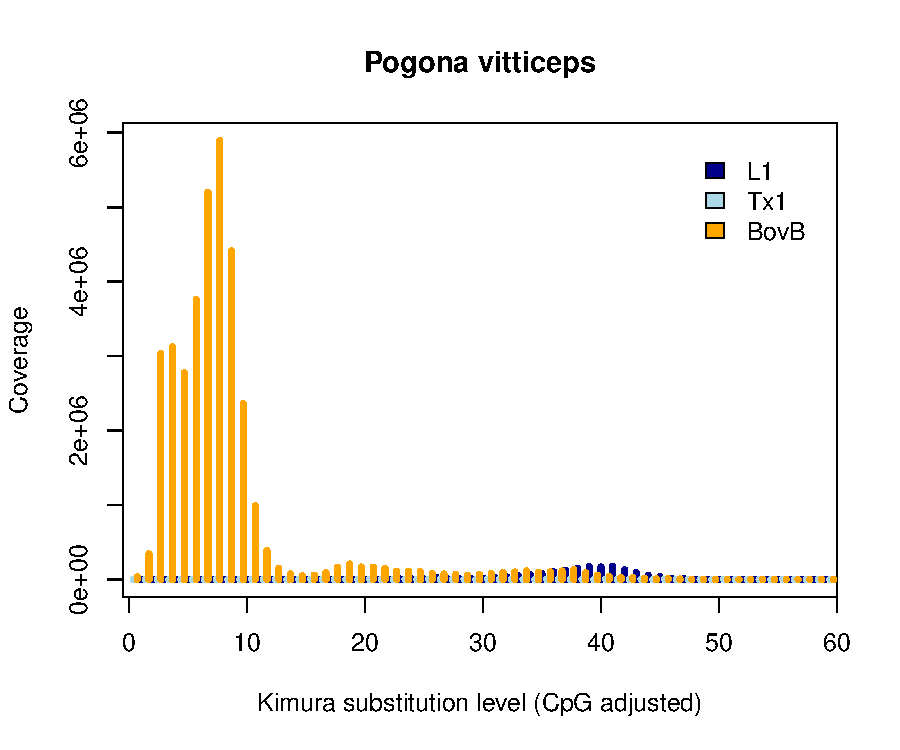
\includegraphics[scale=0.8]{suppFigures/divergencePlots/Pogona_vitticeps.pdf}
	\caption{\label{fig:Pogona_vitticeps}}
\end{figure}

\begin{figure}[H]
	\centering
	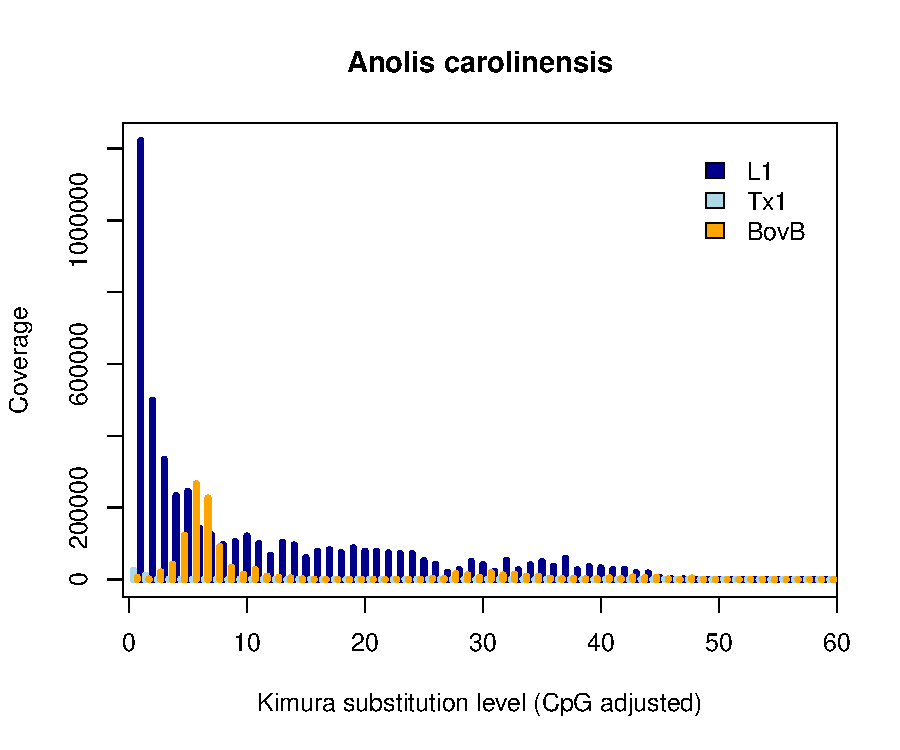
\includegraphics[scale=0.8]{suppFigures/divergencePlots/Anolis_carolinensis.pdf}
	\caption{\label{fig:Anolis_carolinensis}}
\end{figure}

\begin{figure}[H]
	\centering
	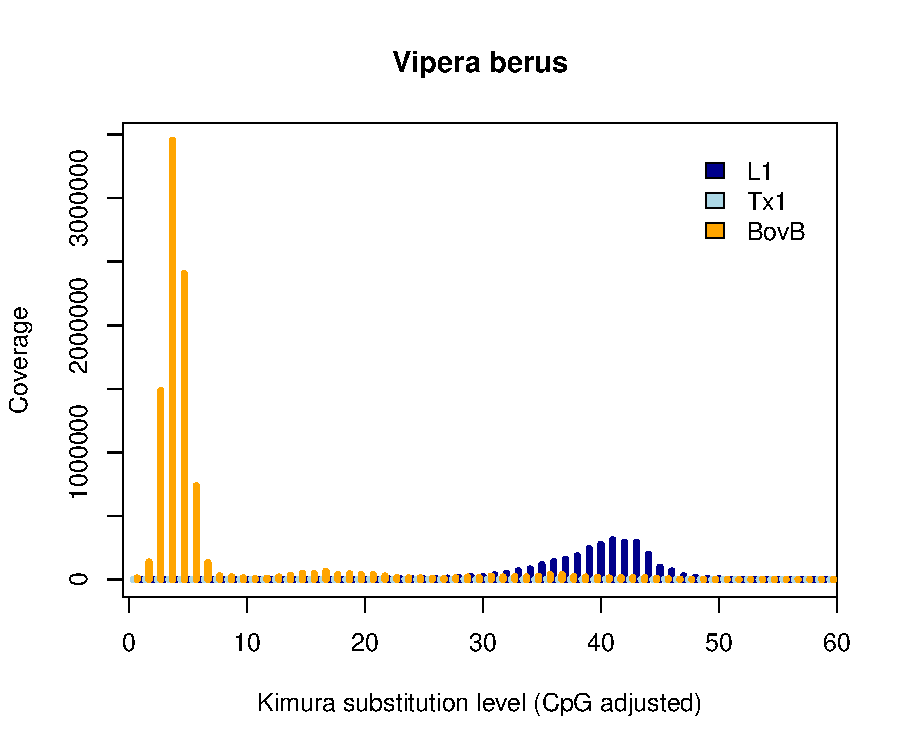
\includegraphics[scale=0.8]{suppFigures/divergencePlots/Vipera_berus.pdf}
	\caption{\label{Vipera_berus}}
\end{figure}

\begin{figure}[H]
	\centering
	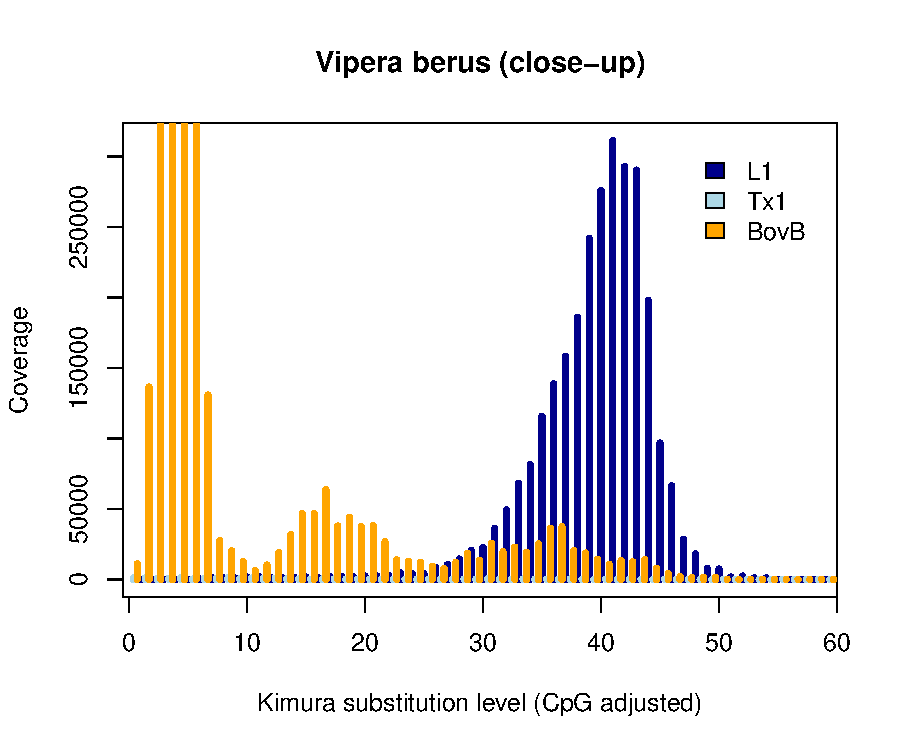
\includegraphics[scale=0.8]{suppFigures/divergencePlots/Vipera_berus_closeup.pdf}
	\caption{\label{Vipera_berus_closeup}}
\end{figure}

\begin{figure}[H]
	\centering
	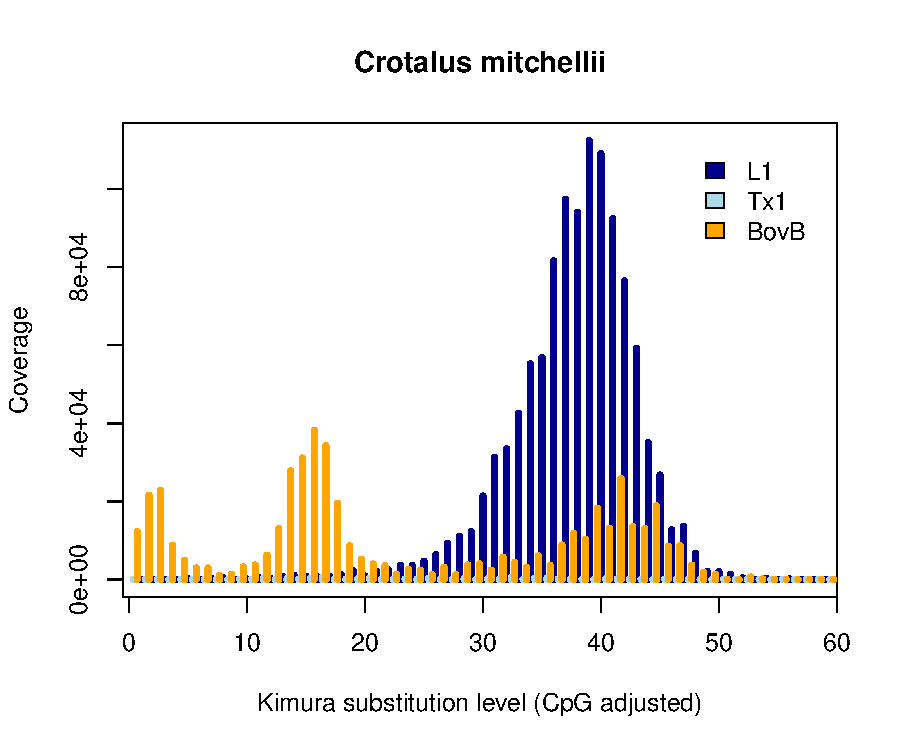
\includegraphics[scale=0.8]{suppFigures/divergencePlots/Crotalus_mitchellii.pdf}
	\caption{\label{Crotalus_mitchellii}}
\end{figure}

\begin{figure}[H]
	\centering
	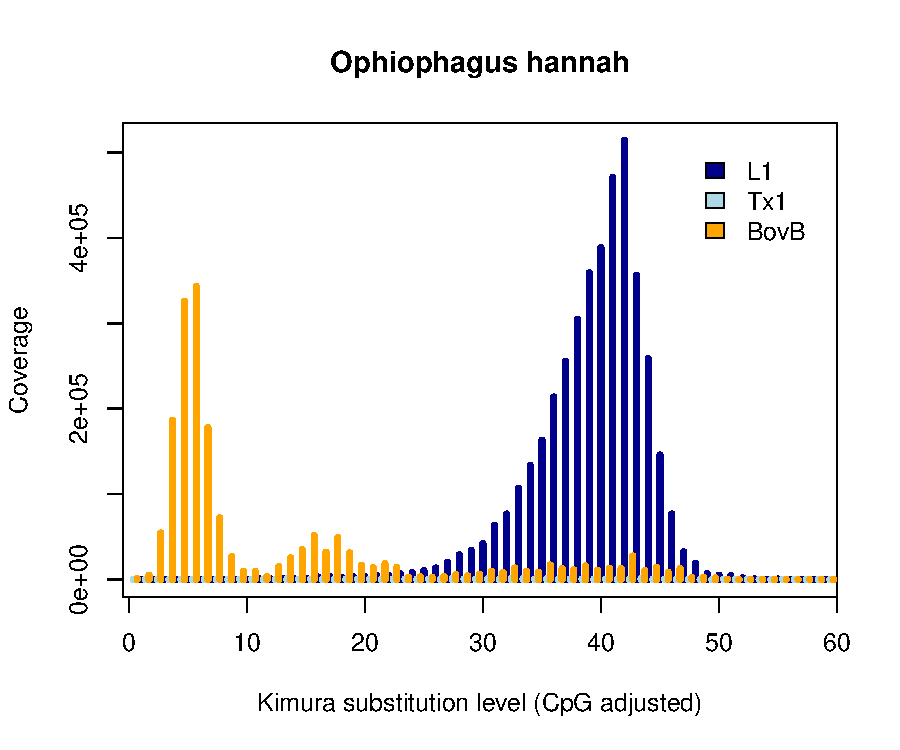
\includegraphics[scale=0.8]{suppFigures/divergencePlots/Ophiophagus_hannah.pdf}
	\caption{\label{Ophiophagus_hannah}}
\end{figure}

\begin{figure}[H]
	\centering
	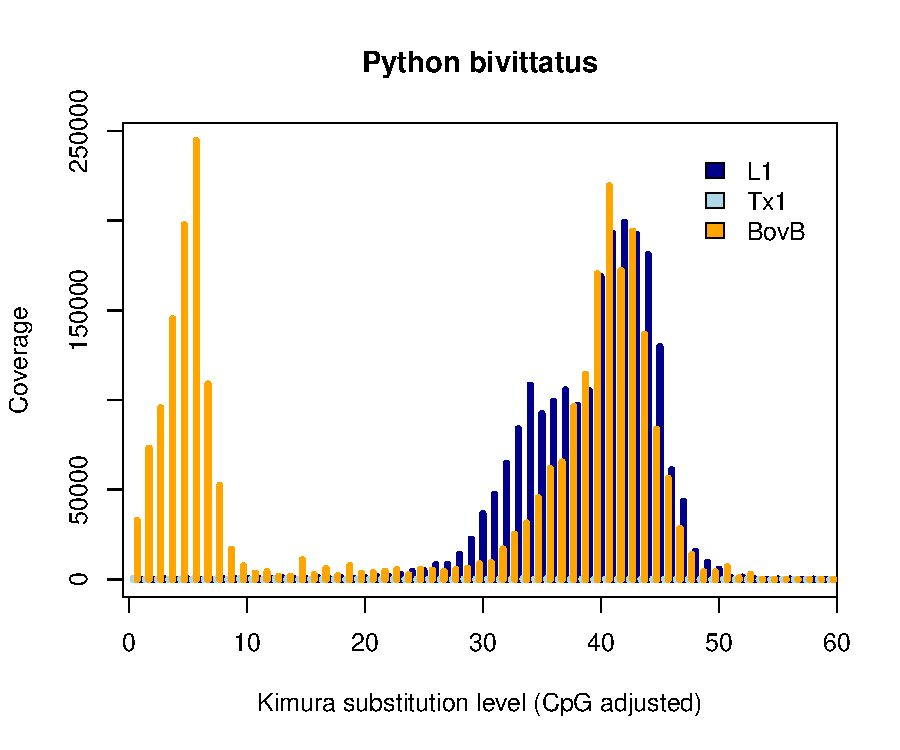
\includegraphics[scale=0.8]{suppFigures/divergencePlots/Python_bivittatus.pdf}
	\caption{\label{Python_bivittatus}}
\end{figure}

\subsection*{Amphibia}
\addcontentsline{toc}{subsection}{Amphibia}

\begin{figure}[H]
	\centering
	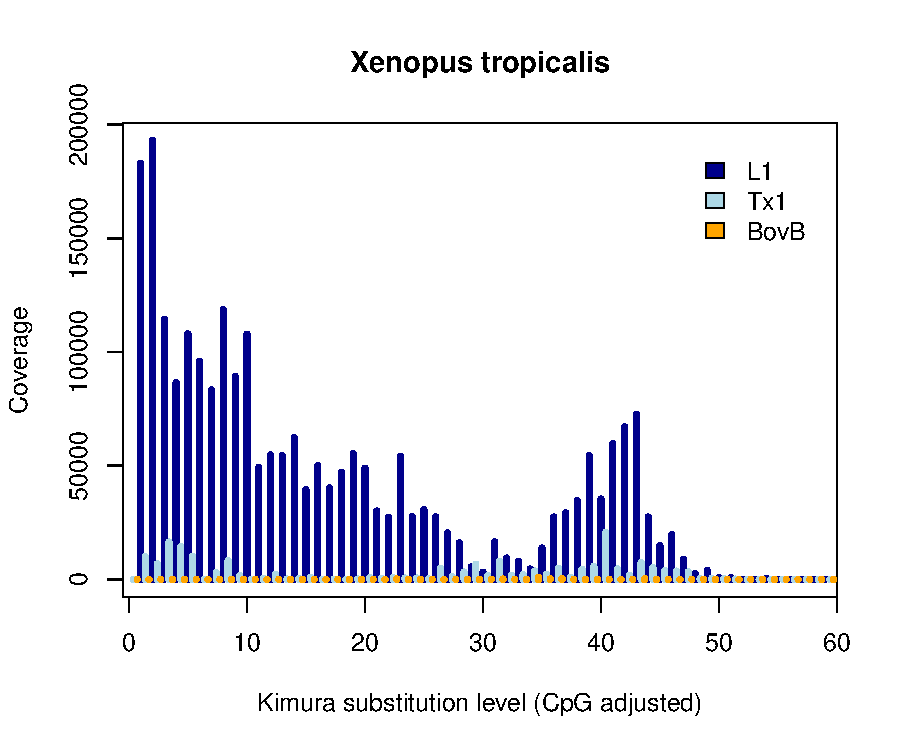
\includegraphics[scale=0.8]{suppFigures/divergencePlots/Xenopus_tropicalis.pdf}
	\caption{\label{Xenopus_tropicalis}}
\end{figure}

\begin{figure}[H]
	\centering
	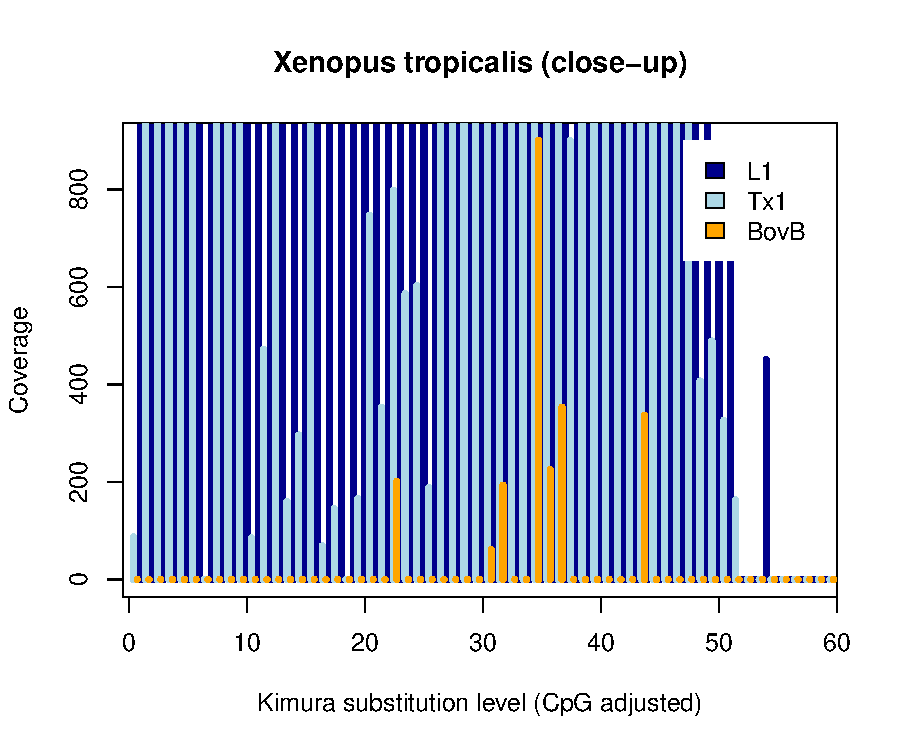
\includegraphics[scale=0.8]{suppFigures/divergencePlots/Xenopus_tropicalis_closeup.pdf}
	\caption{\label{Xenopus_tropicalis_closeup}}
\end{figure}

\subsection*{Neopterygii}
\addcontentsline{toc}{subsection}{Neopterygii}

\begin{figure}[H]
	\centering
	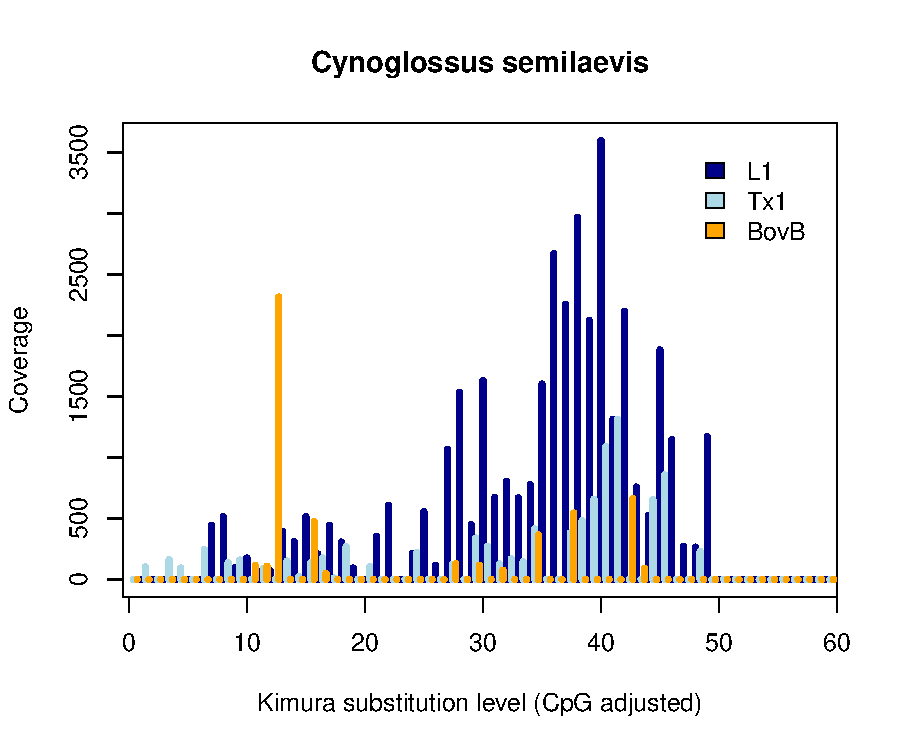
\includegraphics[scale=0.8]{suppFigures/divergencePlots/Cynoglossus_semilaevis.pdf}
	\caption{\label{Cynoglossus_semilaevis}}
\end{figure}

\begin{figure}[H]
	\centering
	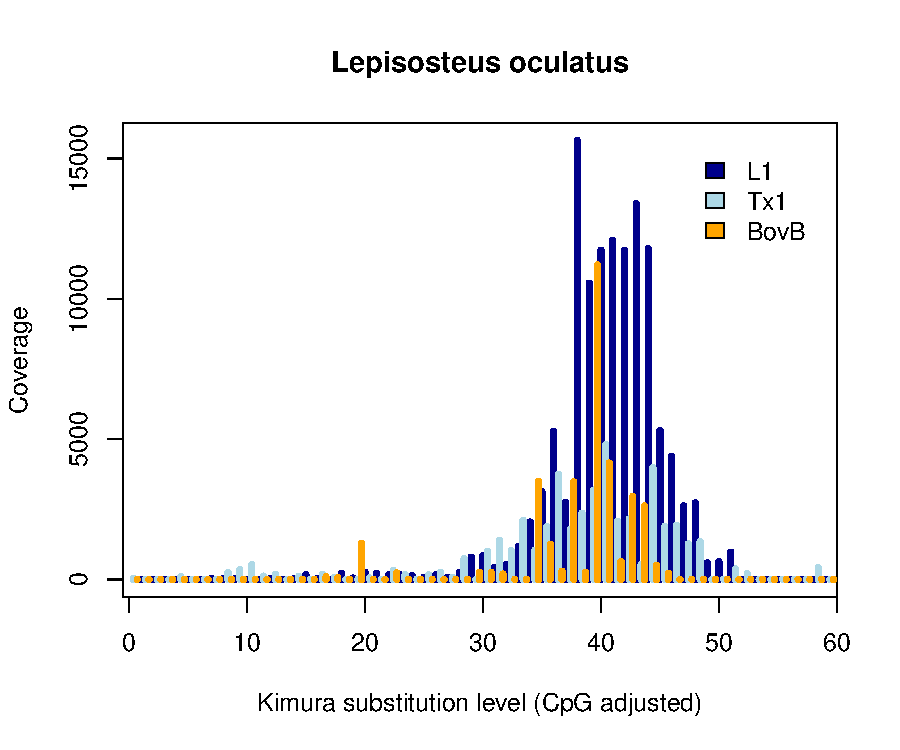
\includegraphics[scale=0.8]{suppFigures/divergencePlots/Lepisosteus_oculatus.pdf}
	\caption{\label{Lepisosteus_oculatus}}
\end{figure}

\begin{figure}[H]
	\centering
	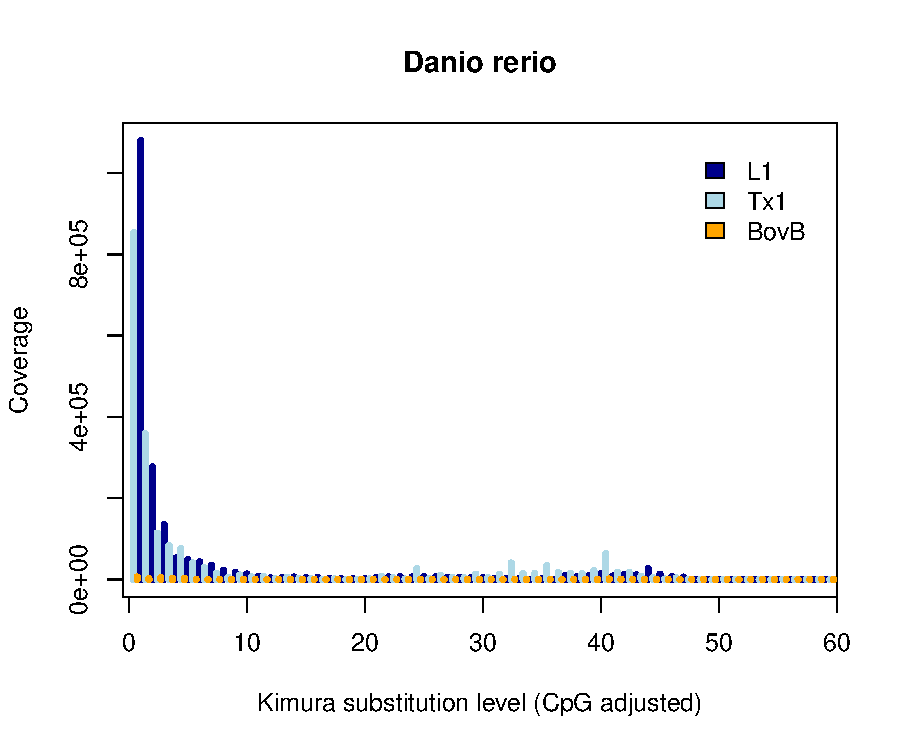
\includegraphics[scale=0.8]{suppFigures/divergencePlots/Danio_rerio.pdf}
	\caption{\label{Danio_rerio}}
\end{figure}

\begin{figure}[H]
	\centering
	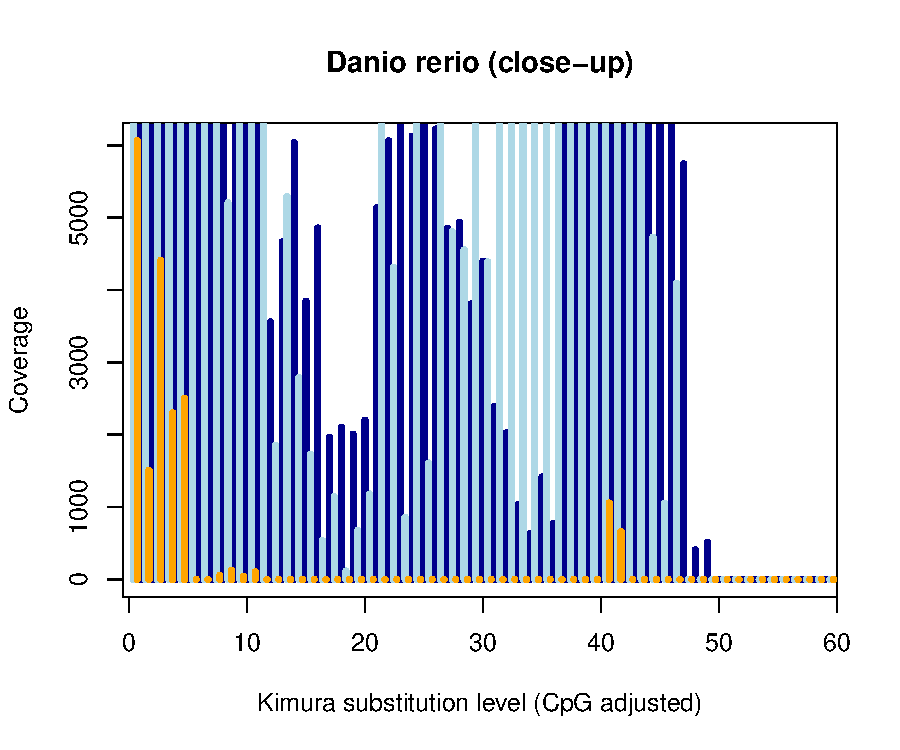
\includegraphics[scale=0.8]{suppFigures/divergencePlots/Danio_rerio_closeup.pdf}
	\caption{\label{Danio_rerio_closeup}}
\end{figure}

\subsection*{Other}
\addcontentsline{toc}{subsection}{Other}

\begin{figure}[H]
	\centering
	\includegraphics[scale=0.8]{suppFigures/divergencePlots/Centruroides_exilicauda.pdf}
	\caption{\label{Centruroides_exilicauda}}
\end{figure}

\begin{figure}[H]
	\centering
	\includegraphics[scale=0.8]{suppFigures/divergencePlots/Helobdella_robusta.pdf}
	\caption{\label{Helobdella_robusta}}
\end{figure}

\begin{figure}[H]
	\centering
	\includegraphics[scale=0.8]{suppFigures/divergencePlots/Strongylocentrotus_purpuratus.pdf}
	\caption{\label{Strongylocentrotus_purpuratus}}
\end{figure}

\begin{figure}[H]
	\centering
	\includegraphics[scale=0.8]{suppFigures/divergencePlots/Ciona_savignyi.pdf}
	\caption{\label{Ciona_savignyi}}
\end{figure}

\section*{Figure S55: Chimeric L1-BovB}
\addcontentsline{toc}{section}{Figure S55: Chimeric L1-BovB}

\begin{figure}[H]
	\centering
	\includegraphics[scale=0.5]{suppFigures/chimeric/rearranged.png}
	\caption{\footnotesize \textbf{Chimeric L1-BovB in cattle genomes. }Several cow ESTs overlap the L1 reverse transcriptase domain, but these may be artifacts/mismapped. No strong evidence to suggest transcription.} \label{Chimeric}
\end{figure}
	
\end{document}
